\documentclass[
bachelor
, english
, a4paper
, 11pt
, oneside
, webreferences
, glossary
, indextop
, acronyms
]{INSOthesis}
\inputencoding{utf8}

\thesistitle{
Optimized native implementation of
Lyra2 password hashing scheme in Java
}
\thesisshorttitle{Lyra2 password hashing scheme in Java}
% \thesissubtitle{}
\thesisdate{\today}

% all titles and designations have to be gender-related!
\thesiscurriculum{
Software Engineering and Internet Computing
}{
Software Engineering and Internet Computing
}
\thesisauthor{Aleksandr Lisianoi}
\thesismatrikelno{01527346}

% advisor
%\thesisauthorpreamble {Verfasser}
%\thesisadvisorpreamble {Betreuung}
\thesisadvisorone {Clemens Hlauschek}
\thesisadvisortwo {Florian Fankhauser}
%\thesisadvisorthree {Vorname Nachname}

% Bibliographie file
\bibliography{bibliography/references}

\hypersetup{
  %colorlinks=false % enable and disable frames around links
}

%%%%%%%%%%%%%%%%%%%%%%%%%%%%%%%%%%%%%%%%%%%%%
%
% Can be used to add additional information
%
%%%%%%%%%%%%%%%%%%%%%%%%%%%%%%%%%%%%%%%%%%%%%
% \AfterTitlePages{}
% \AfterDeclaration{}
% \AfterAcknowledgements{}
% \AfterAbstract{}
% \AfterListOfFigures{}
% \AfterListOfTables{}
% \AfterAbbreviations{}
% \AfterBibliography{}

\renewcommand\afterchapternum{\hspace{1em}}
\begin{document}

\maketitle

%%%%%%%%%%%%%%%%%%%%%%%%%%%%%%%%%%%%%%%%%
%%%   CONTENTS    %%%%%%%%%%%%%%%%%%%%%%%
%%%%%%%%%%%%%%%%%%%%%%%%%%%%%%%%%%%%%%%%%
\setminted{fontsize=\small,baselinestretch=1}

%%%%%%%%%%%%%%%%%%%%%%%%%%%%%%%%%%%%%%%%%%%%%%%%%%%%%%%%%%%%%%%%%%%%%%%%
\chapter{Introduction}
\label{sec:introduction}
%%%%%%%%%%%%%%%%%%%%%%%%%%%%%%%%%%%%%%%%%%%%%%%%%%%%%%%%%%%%%%%%%%%%%%%%
Passwords are currently the backbone of user authentication. Usually, passwords are stored in a hashed form in some kind of a database. Such databases are fairly often compromised and then the hashing mechanism is what stands between the attacker and the password cleartext.

%=======================================================================
\section{Problem Description}
%=======================================================================
Processing power increases with time while simultaneously getting cheaper. This works both for the legitimate users as well as the attackers. Password Hashing Schemes (PHSs) are therefore continuously adjusted to stay irreversible. However, recent advances in highly parallelized hardware (conventional multicore GPUs as well as the more specialized FPGAs and ASICs) present a new challenge for the commonly used cryptographic hash functions. An attacker can heavily parallelize the computation, trying several thousands of password and salt combination in the time it takes a legitimate user to compute just one.

In order to limit the throutput a potential attacker could achieve, the Password Hashing Competition was announced in 2013 and concluded in 2015 \cite{wetzels:2016:phc}. Its evaluation criteria stress that proposed candidates should provide minimal speed-up for the highly parallelized hardware. The winner was declared to be Argon2 \cite{biryukov:2015:argon2} and special recognition was also given to Catena \cite{forler:2013:catena}, Lyra2 \cite{andrade:2016:lyra2,marcos:2015:lyra2}, Makwa \cite{pornin:2015:makwa} and yescrypt \cite{peslyak:2015:yescrypt}.

%=======================================================================
\section{Motivation}
%=======================================================================
Even though the theoretical designs and their proof-of-concept implementations were presented back in 2015, the adoption of these new cryptographic algorithms could be better. There are many ways to do so: provide better documentation, detailed usage examples and success stories. Porting an existing implementation into another programming language can also result in an adoption boost.

%=======================================================================
\section{Contribution}
%=======================================================================
This work describes the porting process of the Lyra2 reference implementation into Java. The resulting implementation is hosted in the Maven central repository \cite{maven:2017:lyra2} as well as on GitHub \cite{github:2017:lyra2-java}. This makes it available for seamless inclusion as a dependency into any Java project. It is licensed under the MIT license which is a well-known permissive software license. Finally, the source code is publicly available and can be inspected or improved if necessary.

The primary goal of this porting effort is to provide a drop-in replacement for the reference implementation. Given the same input parameters, both implementations should produce the same hash values. Although this might sound like an automatic requirement, it is not in fact the case. The paper will highlight the challenges in details about the Java implementation section \ref{sec:java-implementation}.

The secondary goal is to compare the ported implementation to the original. The comparison project is done in the spirit of reproducible research, is hosted publicly on GitHub \cite{github:2017:lyra2-compare} and can be used to verify the results presented in this paper.

The final goal is to use the ported implementation to write an Android application. Section \ref{sec:mobile-application} demonstrates the ease of deployment of Lyra2 on a platform where using the reference implementation is not as straightforward.

%=======================================================================
\section{Outline of the Work}
%=======================================================================

\emph{Section \ref{sec:fundamentals}} is devoted to theoretical background. It opens with the basic definitions as well as a brief mention of existing password hashing solutions which are either not memory-hard or have other notable drawbacks. A short description of Lyra2 follows in \ref{sec:lyra2-brief-description}, introducing the notion of a sponge function as well as a duplex construction. The main part of that section deals with the memory matrix created by Lyra2 and the way it interacts with the duplex constructions during the different phases of the algorithm.

\emph{Section \ref{sec:implementation-details}} covers implementation details. It begins with a quick discussion of the reference implementation \ref{sec:reference-implementation}. It outlines the build system and the various possible configurations of Lyra2. The section concludes with an extension of the build system which allows to compile several configurations at once as well as compute a bulk of hash values. The ported Lyra2 project is discussed next in \ref{sec:java-implementation}. It first deals with the transition from a function-based to an object-oriented project. The most important classes are shown on an UML diagram \ref{fig:uml}. Several classes exist to circumvent specific porting challenges. These challenges are explained and illustrated. In particular, the endianness issue is shown in figure \ref{fig:little-endian} and a rotation trick for the Blake2b-based sponge is shown in figure \ref{fig:sponge-blake2b}.

\emph{Section \ref{sec:results}} summarizes the results. It begins with the demonstration that both projects produce the same hash values given the same inputs \ref{sec:it-works}. First, a manual testing session is recorded in \ref{sec:manual-testing}. A section on continuous integration follows in \ref{sec:automated-testing}. Then the performance comparison is presented in section \ref{sec:performance-comparison}. Due to a large number of configurable parameters in Lyra2, the first comparisons fix time- and memory costs (respectively, subsections \ref{sec:fixed-time-cost} and \ref{sec:fixed-memory-cost}). Section \ref{sec:no-fixed-costs} then deals with both changing time- and memory costs, resulting in several thousands of measurements displayed. A comparison conclusion is made in \ref{sec:comparison-conclusion}. Finally, an Android mobile application is presented in \ref{sec:mobile-application}.

\chapter{Related Work}
\label{chapter:related-work}

As mentioned in Chapter \ref{sec:introduction}, this paper describes three stages during which a user's credentials must be protected. In particular, Section \ref{sec:secure-authentication} describes secure authentication, Section \ref{sec:secure-communication} covers secure communication and Section \ref{sec:secure-password-storage} discusses secure password storage. Each section provides an overview of common threats as well as defensive techniques. The chapter culminates with an introduction to memory-hard password hashing algorithms.

\section{Secure Authentication}
\label{sec:secure-authentication}

This section presents a brief overview of different methods for secure authentication and some of the accompanying types of attacks. The presented taxonomy was in part borrowed from Raza et al. \cite{raza:2012:password-attacks-survey} and then expanded and filled with details from other sources.

\subsection{Authentication Approaches}
\label{sec:authentication-approaches}

Several authentication approaches have emerged over the years. Some of them are really widespread and quite old.  At the same time others are rather novel and aim to overcome known issues. Below is a list of common authentication schemes.

\emph{Conventional Passwords} are by far the most common method of user authentication \cite{bonneau:2015:passwords-and-evolution-of-auth}. The service challenges the user to produce a pair of a (public) username and a (private) password. If the provided pair is correct, the user is allowed to proceed, otherwise the request is rejected. Such an intuitive approach works reasonably well but there are a number of fundamental issues.

 According to sources from Ives, Walsh and Schneider \cite{ives:2004:domino}, a typical user daily accesses roughly 15 services that require a password. At the same time, the user remembers on average 5 unique passwords. This suggests that some of those passwords are reused for several services. Even if attempts are made to slightly tailor the password to the service, this reuse still has a devastating effect on security, as shown by Gaw and Felten in \cite{gaw:2006:password} or Shay et al. in \cite{shay2010encountering}. The most protected account becomes as secure as the least protected one and the possibility of a breach grows with the number of services that share the same (or a similar) password.

Conventional passwords have been shown to have many flaws, see e.g. Yan et al. \cite{yan:2004:password}, Braz and Robert \cite{braz:2006:security} or Jobusch and Oldehoeft \cite{jobusch:1989:survey-of-password-mechanisms-1, jobusch:1989:survey-of-password-mechanisms-2}. Therefore it is not surprising that a number of viable alternatives has been developed over the years.

\emph{Graphical Passwords} are one such alternative. They can generally be subdivided into two categories: recognition and recall based, as done by Suo, Zhu and Owen in \cite{suo:2005:graphical-passwords-survey}. The \emph{recognition based} graphical passwords vary widely, the main idea being that the user has to recognize correct images and perform an action. For example, clicking on previously chosen pictures or clicking inside a convex hull created by them. Pictures of human faces are sometimes suggested because they are arguably the easiest to remember but other types of imagery are used as well. The \emph{recall based} schemes, on the other hand, expect the user to reproduce some type of a drawing. These include the well-known graphical passwords on smartphones, where the user is typically required to connect points of a \(3 \times 3\) grid with straight lines without lifting the finger off the screen. More complex approaches either let the user initiate several touch gestures (thus producing an even more detailed drawing) or write something that resembles a signature.

Some applications of graphical passwords claim better resistance to shoulder surfing attacks \cite{suo:2005:graphical-passwords-survey}. Unfortunately, these schemes usually take more time on average to perform the login when compared to conventional passwords. This adversely affects their practical application.

\emph{Keystroke Dynamics} is an elegant authentication mechanism, described e.g. by Monrose and Rubin \cite{monrose:2000:keystroke-dynamics}, which tries to capture the typing pattern of a legitimate user. Several statistics about the speed and rhythm, with which the user presses the keys, are captured: the time between consecutive keys, the time between pressing and releasing the key, the time it takes to type certain words etc. A more extensive list of metrics can be found in  Tillmann, de Halleux and Xie \cite{teh:2013:survey-keystroke-biometrics}. Those statistics are then used in a machine learning algorithm which ultimately decides if the user passes authentication or gets rejected. These algorithms include fine-tuned \(k\) Nearest Neighbors, as shown i.e. by Ivannikova, David and Hämäläinen \cite{ivannikova:2017:anomaly-detection-keystroke-dynamics}, naïve Bayes, as in Ho and Kang \cite{ho:2017:onenb}, gaussian mixture models, as in Deng and Zhong \cite{yunbin:2013:gmm-keystroke}, and others.

An immediate challenge is that in this scenario authentication becomes \emph{probabilistic}. Instead of asking "what the user knows", methods based on keystroke dynamics evaluate "what the user is" by judging their ability to type. This is particularly difficult in edge cases when the user is under heavy mental stress or is somehow physically restricted. One possible solution is to perform authentication as a continuous process, as shown in Borus \cite{bours2012continuous} or Serwadda et al. \cite{serwadda2013scan}. In such a scenario the user is monitored over a prolonged period of time. Similar challenges also appear with a few other biometric authentication methods, of which keystroke dynamics is a prominent example.

\emph{Biometric Authentication} is a collective term for a technique which focuses on physical traits unique to every user, as explained by e.g. Matyas and Riha \cite{matyas:2003:toward}. These include fingerprints, facial recognition, voice recognition, iris scanning and similar. Other types of biometric data as well as certain challenges connected with false recognition and false non-recognition can be found in Jain, Ross and Prabhakar \cite{jain:2004:intro-to-biometric}. That paper also highlights the notion of \emph{negative recognition} which means that biometric authentication allows to establish if the person is who they \emph{deny} to be. This property distinguishes this class of methods from all the others described in this section.

\emph{One-time Passwords} is another elegant solution for user authentication. As defined by Rayes \cite{rayes:2005:otp}, it is a password that is used exactly once and then immediately discarded. Such a password is usually used in a multi-factor fashion, specifically \gls{2fa}. This means that the user first provides the conventional username/password pair ("what the user knows") and then follows it up with a one-time password. This second password is expected to come from a dedicated smart card, a separate keyfile or a smartphone application ("what the user has"). Of major interest are two one-time password generation algorithms: \gls{hotp}, specified by M’Raihi et al. \cite{rfc4226}, and \gls{totp}, also by M’Raihi et al. \cite{rfc6238}. They are both designed as part of the \gls{oath}. The demand for such algorithms as well as a system that uses conventional smartphones for \gls{2fa} was demonstrated for example by
Aloul, Zahidi and El-Hajj \cite{aloul:2009:two-factor-auth}.

\subsection{Conventional Password Strength}
\label{sec:password-strength}

Previous Section \ref{sec:authentication-approaches} describes several approaches to user authentication. It mentions that conventional passwords are the most widespread means of user authentication \cite{bonneau:2015:passwords-and-evolution-of-auth}. That section also shows that conventional passwords have their set of problems \cite{yan:2004:password, braz:2006:security, jobusch:1989:survey-of-password-mechanisms-1, jobusch:1989:survey-of-password-mechanisms-2}. Therefore, being able to distinguish between strong and weak passwords is important. Several methods to do so are presented below.

\emph{Information Entropy} is the usual way to assess password strength, consult e.g. Bonneau \cite{bonneau:2012:the-science-of-guessing}. It is a base-two logarithm of the number of guesses which are required to recover a password with complete certainty. Information entropy is measured in bits. For example, if the password is completely random and has \(x\) bits of information entropy, then an attacker must compute \(2^x\) password candidates to be guaranteed a successful recovery.

Human generated passwords, however, are notorious for not being truly random. Which is why computing information entropy often produces inaccurate results \cite{bonneau:2012:the-science-of-guessing}.

\emph{NIST Special Publication 800-63-2} by Burr et al. \cite{burr2013electronic} tried to address this problem and suggested a refined way of computing information entropy for passwords:

\begin{itemize}
    \item The entropy of the 1\textsuperscript{st} character is 4 bits.
    \item The entropy of characters 2 to 7 is 2 bits per character.
    \item The entropy of characters 9 to 21 is 1.5 bits per character.
    \item The entropy of characters 21 and above is 1 bit per character.
    \item If \emph{both} uppercase letters and non-alphabetic characters are used, the password gains 6 more bits of entropy.
    \item If the password is 1 to 19 letters long and passes an extensive dictionary check, then an additional 6 bits of entropy should be added.
  \end{itemize}

The last bonus is not assigned to passwords of length 20 and above because it is assumed that those are \emph{pass phrases}, i.e. passwords which consist of several dictionary words. This refined approach was still criticized for being inaccurate and was removed from the revised version of the publication by Grassi, Garcia and Fenton \cite{grassi2017digital}.

\emph{Guess Number Calculation} is a different approach to estimating password strength suggested by Kelley et al. \cite{kelley2012guess}. The idea behind this method is to first choose a particular algorithm for password cracking which is known to work well. The number of password candidates which this algorithm needs to try before recovering the target password becomes the indicator of this password's strength. Such an approach was shown to perform reasonably well but it also comes with its own challenges, as pointed out by Weir et al. \cite{weir2010testing} or Zhang, Monrose and Reiter \cite{zhang2010security}. First of all, the choice of the algorithm is arbitrary. Secondly, many state of the art password cracking algorithms require a training set to fine tune their parameters. Changing the training set essentially produces a different configuration of the algorithm. This in turn leads to a recalculation of guess numbers. So, this approach in general is mainly empirical and often volatile.

\subsection{Authentication Attacks}
\label{sec:authentication-attacks}

Previous sections, namely Section \ref{sec:authentication-approaches} and Section \ref{sec:password-strength}, describe authentication approaches and password strength estimation. Section \ref{sec:authentication-attacks} provides a summary of some of the common types of authentication attacks.

\emph{Brute Force} is the most common and least sophisticated type of a password attack, see e.g. Narayanan and Shmatikov \cite{narayanan:2005:fast}. The attacker begins by choosing a specific password domain and then launches the trial and error guessing process. For example, one could try all passwords that are up to 8 characters in length and consist of lowercase Latin letters. This domain contains \(217180147158\) unique passwords. Assuming that the attacker can try \(1000\) passwords per second, it will take them \(\approx 6.8\) years to complete the search. This might sound like a lot of time but the \(1000\) passwords per second is a conservative speed estimate. Depending on the available hardware, the hash algorithm and other factors, this speed could be a \emph{a lot} higher. Table \ref{table:hashcat-speed} shows some real world speeds for a few password hashing algorithms as measured by running a common hash computation tool on ordinary consumer hardware available to the author of this paper.

\begin{table}
    \begin{center}
        \begin{tabular}{lr}
            Hashtype & Millions of hashes per second \\
            \hline
            MD5 & 2912.4 \\
            SHA1 & 1004.6 \\
            SHA-512 & 117.6 \\
            SHA-3 (Keccak) & 104.6
        \end{tabular}
    \end{center}
    \caption{Hashcat v3.6.0 Running on a Single Nvidia GTX 950M Graphics Card}
    \label{table:hashcat-speed}
\end{table}

\emph{Dictionary Attacks} are an improvement upon brute force \cite{narayanan:2005:fast}. A dictionary is a collection of possible passwords, often ordered by popularity or likelihood of occurrence. Such dictionaries are compiled from various sources: conventional language dictionaries, website pages, previously leaked passwords and so on. Advanced dictionaries or software that uses them often include \emph{mutations}. A mutation is a modification rule applied to a dictionary entry. An example of a popular modification rule might be a substitution of the letter \(o\) with the digit \(0\) or an addition of \(42\) to the end of the password. Dictionary attacks with modification rules are the most common academic approach to password cracking \cite{zhang2010security, weir2010testing, kelley2012guess, shay2010encountering}.

Even though dictionary attacks are the standard go-to method for password recovery research, there are several problems with this approach \cite{bonneau:2012:the-science-of-guessing}. Rather often it is difficult or outright impossible to accurately compare the results of different studies. For example, the exact password dictionaries may not be available to every researcher because they must be purchased or have changed since the date of the study. The popular tools used for the analysis are also being constantly developed, so keeping track of the exact versions is cumbersome \cite{bonneau:2012:the-science-of-guessing}.

\emph{Markov Model Based Attacks} are an example of machine learning techniques applied to password recovery, consult e.g. Dell’Amico, Michiardi and Roudier \cite{dell:2010:password}. When constructing the next password candidate, these algorithms use the beginning of the string to determine its end. For example, if the first part of the password candidate is "deter", then the Markov model will try "determine" and "detergent" earlier than "deteraaa" or "deter000". The algorithm uses training data to fit a probability distribution over the domain of possible passwords. Once the distribution is constructed, the most probable password candidates are tried first, which in practice noticeably increases the speed of password recovery. An interesting observation made by the authors of \cite{dell:2010:password} is that the second-best training data is the collection of usernames. The best training set is the passwords themselves. In other words, training a Markov model on the usernames and then using it to recover the passwords works very well. This is an intriguing observation because the password and the username are supposed to serve different purposes. The provided explanation is that the user creates both the password and the username during registration in quick succession. This is why many users probably reuse the same thinking patterns and ideas to come up with these two strings.

\emph{Shoulder Surfing} is an entirely different kind of a password attack \cite{raza:2012:password-attacks-survey, suo:2005:graphical-passwords-survey} . As the name suggests, its simplest form is a person standing next to the user who is performing authentication. However, this is by far not the only scenario. The user might be authenticating from a café, a bank, an airport or any other location with sufficiently advanced video surveillance system. If a high resolution recording of the user's authentication process is captured, then this video becomes a viable attack vector.

\emph{Phishing Attacks} are yet another formidable type of an attack, as summarized by Hong \cite{hong:2012:state} or Wu, Miller and Garfinkel \cite{Wu:2006:STA:1124772.1124863}. A legitimate user is usually tricked into visiting a webpage which impersonates a typical webservice, like an e-mail provider or a social network. The user is then prompted to enter their authentication details. If they do not recognize the attack in time then their credentials end up in the hands of the attackers. Phishing attacks usually target a large group of individuals and do not use personalized information. On the other hand, \emph{spear phishing attacks} is a term reserved for targeting specific people (journalists, politicians, high-profile executives, etc.) \cite{hong:2012:state}. These attacks are a lot harder to defend from because the information is tailored specifically to the target.

\section{Secure Communication}
\label{sec:secure-communication}

Previous Section \ref{sec:secure-authentication} is devoted to the authentication stage. Current Section \ref{sec:secure-communication} discusses the next stage, namely communication. In particular, the question of establishing a secure communication channel over an insecure connection is addressed.

\subsection{Secure Sockets Layer and Transport Layer Security}
\label{sec:ssl-tls}

\emph{\gls{ssl}}, as standardized by Freier, Karlton and Kocher \cite{rfc6101}, and \emph{\gls{tls}}, as formalized by Dierks and Rescorla \cite{rfc5246}, are a pair of protocols widely used to ensure secure communication. \gls{tls} first appeared in 1999 and is the successor to \gls{ssl}. The \gls{tls} protocol guarantees that the connection between communicating parties is \emph{secure} (i.e. a passive eavesdropper will not obtain information) and \emph{reliable} (i.e. an active attempt to tamper with the connection will be detected). The authentication of communicating parties can occur with the help of \emph{public key cryptography}. With a bit of additional configuration \emph{forward secrecy} can be achieved as well, as shown by Adrian et al. \cite{Adrian:2015:IFS:2810103.2813707}. Forward secrecy means that if at some later point the service is compromised and its private keys are leaked, the contents of the past communication sessions will not be affected.

TLS is a complex algorithm which allows \emph{a lot} of flexibility when it comes to parameter choice. It begins with a TLS \emph{handshake}:

\begin{enumerate}
    \item The client presents the list of supported ciphers and hash functions to the server.
    \item The server chooses a cipher and hash function and informs the client.
    \item Usually, the server also provides identity information by means of a digital certificate.
    \item The client decides if they want to proceed based on identity information (or lack thereof).
    \item The client and the server generate a unique session key: if perfect forward secrecy is required, then a variation of a Diffie-Hellman key exchange takes place. Otherwise, the client generates a random number and encrypts it with the server's public key. Once passed to the server, it will be decrypted with the server's private key.
  \end{enumerate}

During the handshake different algorithms can be negotiated: \gls{rsa}, Diffie-Hellman, ephemeral Diffie-Hellman, Elliptic Curve Diffie-Hellman, ephemeral Elliptic Curve Diffie-Hellman, and a few others. The digital certificate relies on the \emph{\gls{pki}} which consists of users as well as registration and certificate authorities (RAs and CAs respectively). PKI in general receives a lot of criticism:

\begin{itemize}
    \item Obtaining a digital certificate costs both time and money.
    \item CAs are being constantly breached which enables attackers to issue fake certificates: the 2011 Comodo \cite{comodo:2017:ca-incident} and DigiNotar \cite{diginotar:2017:ca-incident} incidents, the 2013 ANSSI \cite{anssi:2017:ca-incident} and TURKTRUST \cite{turktrust:2017:ca-incident-0} incidents, the 2014 National Informatics Center of India \cite{nic:2017:ca-incident} incident, the 2015 \& 2016 loss of trust in Symantec \cite{symantec:2017:ca-incident-0, symantec:2017:ca-incident-1}, 2016 \& 2017 loss of trust in WoSign and StartCom \cite{startcom:2017:ca-incident-0, startcom:2017:ca-incident-1}.
    \item Protocol versions are known to have been deprecated due to design flaws and security vulnerabilities. SSL 2.0 was formally deprecated by Polk and Turner \cite{rfc6176}, SSL 3.0  --- by Barnes et al. \cite{rfc7568}. TLS 1.2 is the current latest version of the protocol.
    \item Libraries that implement the protocol have had major security issues. One of the most well-known examples is \emph{Heartbleed}, as described by Durumeric et al. \cite{durumeric2014matter}. It was a major vulnerability that existed between 2012 and 2014 in a widely used OpenSSL library. The bug allowed anyone access to arbitrary data as a result of a buffer overflow.
  \end{itemize}

The list of incidents and issues is by no means complete. However, \gls{ssl} and \gls{tls} are an ubiquitous pair of protocols which have been in use for a long time. Therefore, it should not come as a surprise that a few design and usage problems have surfaced over the years. The lack of trust in certificate authorities remains a cornerstone design issue though. This lead to the development of a number of alternative secure communication methods that do not rely on the current \gls{pki}. One such family of methods is described next in Section \ref{sec:pake}.

\subsection{Password Authenticated Key Exchange}
\label{sec:pake}

\emph{\gls{pake}} is a family of methods that establish secure communications over an insecure channel without the need for a \gls{pki}. Insight into a select couple of protocols is provided below. In each case the described protocols provide the following guarantees:

\begin{enumerate}
    \item Resistance to offline dictionary attacks.
    \item Resistance to online dictionary attacks: only one password attempt per session.
    \item Forward secrecy: past and current session keys remain secure if the password is compromised at some later point in time.
    \item Known session key security: past and future sessions remain secure even if the current session key is compromised.
  \end{enumerate}

\emph{\gls{eke}}, pioneered by Bellovin and Merritt \cite{bellovin1992encrypted, bellovin1993augmented}, was the first method from the \gls{pake} family. Its early version consists of the following steps (where Alice and Bob are the names of participating parties):

\begin{enumerate}
    \item Alice and Bob both know a (weak) conventional password \(P\).
    \item Alice begins by generating a random public/private pair of keys \(E_A\) and \(D_A\). She uses \(P\) to encrypt the public key: \(M_0 = P(E_A)\). She sends \(M_0\) to Bob.
    \item Bob uses \(P\) to decrypt the public key of Alice: \(P^{-1}(P(E_A)) = E_A\). He then generates a random secret key \(R\) and encrypts it first with the asymmetric and then with the symmetric keys: \(M_1 = P(E_A(R))\). Then he sends \(M_1\) to Alice.
    \item Alice uses both \(P\) and \(D_A\) to recover \(R\): \(D_A(P^{-1}(P(E_A(R))) = R\).
  \end{enumerate}

Once this initial exchange is over, both Alice and Bob know \(R\) and \(E_A\), which are presumed to be stronger than the initial (weak) conventional password \(P\). Better strength is presumed because both \(R\) and \(E_A\) are supposed to have been generated randomly over a large possible keyspace. If the attacker controls the communication channel, then they know \(M_0 = P(E_A)\), \(M_1 = P(E_A(R))\) and \(R(\texttt{Known message})\). To try some candidate password \(P'\), they must produce a candidate \(E_A^{'} = P^{'-1}(P(E_A))\) and then decide if there exists a key \(R'\) such that \(E'_A(R') = E_A(R)\) and \(R^{'-1}(R(\texttt{Known message}))\) recovers the known message. This is expected to be far more expensive than a plain attack on \(P\).

The straightforward implementation of EKE was shown to be insecure by Hao and Ryan \cite{hao2010j}. In addition to that it is patent-encumbered. Therefore, alternative protocols have been developed.

\emph{\gls{jpake}} is a more recent and advanced method from the PAKE family \cite{hao2010j}. It has a formal security proof provided by Abdalla, Benhamouda and MacKenzie \cite{abdalla2015security}. Its computation cost is similar when compared to EKE. Moreover, it is not patented and has been included into such cryptographic libraries as OpenSSL and Bouncy Castle.

\section{Secure Password Storage}
\label{sec:secure-password-storage}

Section \ref{sec:secure-authentication} and Section \ref{sec:secure-communication} discussed methods for secure authentication and communication. The rest of this work focuses on the problem of secure password storage. This issue is as important as the ones discussed above because password databases are routinely compromised \cite{dell:2010:password, bonneau:2012:the-science-of-guessing, ives:2004:domino}. As a result, protection against offline dictionary attacks is of utmost importance.

\subsection{Cryptographic Competitions}
\label{sec:cryptocomps}

It is common practice to announce a competition in order to develop standard cryptographic primitives. For example, the symmetric block cipher Rijndael by Daemen and Rijmen \cite{daemen:2002:DRA} was chosen to become the Advanced Encryption Standard (AES) \cite{aes-fips} in a competitive selection process \cite{nist:1997:aes-development, nist:2017:aes-development} that lasted from 1997 to 2000. The competition was organized by the \gls{nist} and included 15 different designs which were narrowed down to 5 during the final phase: Rijndael \cite{daemen:1998:rijndael}, Serpent by Biham, Anderson and Knudsen \cite{anderson:1998:serpent}, Twofish by Schneier et al. \cite{schneier:1998:twofish}, RC6 by Rivest et al. \cite{rivest:1998:rc6} and MARS by Burwick et al. \cite{burwick:1998:mars}. Another competition was held by \gls{nist} between 2007 and 2012 in order to select the next hash function standard, \gls{sha3}. The final round included 5 designs: Blake by Aumasson et al. \cite{aumasson:2013:blake2}, Grøstl by Gauravaram et al. \cite{praveen:2011:groestl}, JH by Wu \cite{wu:2011:jh}, Skein by Ferguson et al. \cite{ferguson:2009:skein} and Keccak by Bertoni et al. \cite{cryptoeprint:2015:keccak}, the last of which ultimately became the winner of the competition.

Choosing cryptographic primitives through an open competitive process is an effective approach. Therefore, when the need for an updated, memory-hard \gls{phs} became apparent, a Password Hashing Competition was held. This time, however, it was not organized by NIST but directly by the cryptographic community. In particular, the \url{password-hashing.net} (visited on 10/28/2017) website lists two well-known cryptographers Khovratovich and Aumasson as direct contacts. The Password Hashing Competition concluded in 2015, with Argon2 \cite{biryukov:2015:argon2} selected as its winner and Catena \cite{forler:2013:catena}, Lyra2 \cite{andrade:2016:lyra2}, Makwa \cite{pornin:2015:makwa} and yescrypt \cite{peslyak:2015:yescrypt} receiving special recognition.

\subsection{Password Hashing Fundamentals}
\label{sec:fundamentals}

\emph{Password hashing} is the process of transforming a password into a hash value. Given the resulting hash value, it should be computationally infeasible to restore the original password.

Password hashing is common practice when user authentication is required. The user provides a password which is then hashed using some password hashing algorithm. The resulting hash is then compared against a hash value which is stored in the database and is known to be correct. If both hashes match, the user is authenticated.

When a password database is leaked, the password hashing process is what prevents the attackers from gaining the original plaintext passwords. One of the early \glsentrylongpl{phs}, which is widely used today, is PBKDF2, described in section 5.2 of the \gls{rfc} specification by Moriarty, Kaliski and Rusch \cite{moriarty:2017:pkcs}. The fundamental idea behind it (which is shared among a few other early \glsentrylongpl{phs}) is to apply a \emph{pseudo-random function} a number of times, treating the number of repetitions as a parameter for computational cost.

One of the early kinds of attacks against password hashes were \emph{rainbow tables}, as discussed by Avoine, Junod and Oechslin \cite{Avoine:2008:CIT:1380564.1380565}. They are a classic example of a \emph{\gls{tmto}} \cite{Avoine:2008:CIT:1380564.1380565}. Given a dictionary of possible passwords (up to a certain length and using a particular set of symbols) and a hashing algorithm, an attacker precomputes hash values well in advance. When a password database of the defender is leaked, the hash values are compared to those from the rainbow table. If two hashes match, the recovery of the original password becomes a matter of a simple lookup.

The currently well-known defense against the rainbow table attack is to use a sufficiently large \emph{salt} when computing the password. This salt is a randomly generated value which is unique for every password and is openly stored alongside it in the defender's database. The salt ensures that the attacker will have to perform the computation after the leak (possibly giving a chance to the defender to change their password). Another nice property is that the same password used by several users will be very likely to produce distinct hash values.

These days an attacker can often compute a large number of hashes in parallel, as shown by Murakami, Kasahara and Saito \cite{5665047}. If so, the increased individual computational time cost of one hash does not prevent the attacker from trying many candidates at once. The throughput of the attack (average attempted passwords per second) remains high. This type of attacks is addressed by memory-hard \glsentrylongpl{phs}. The main idea is that parallel systems (such as general-purpose \glspl{gpu} or specialized \glspl{asic} and \glspl{fpga}) usually have significantly less memory per one processing unit than \glspl{cpu} of a personal computer. Therefore, if a password hashing process offers a memory cost parameter, an attacker will need (much) more memory per each specialized processing unit in order to have the same throughput. This is supposed to make the attack much more expensive and slow it down considerably.

Arguably the first \gls{phs} to implement this idea was scrypt by Percival \cite{percival:2016:scrypt}, which was recently published as \mbox{\gls{rfc} 7914} by Percival and Josefsson \cite{rfc7914}. However, this scheme is sometimes criticized for being overly complicated and not offering a decoupled way to control time and memory costs. In other words, there is a single parameter that controls both those values.

In order to create new designs which would address the need for a new memory-hard password hashing function, the Password Hashing Competition was announced in 2013 and concluded in 2015 \cite{wetzels:2016:phc}. Below follows a quick summary of its winner (Argon2 \cite{biryukov:2015:argon2}) and all of the finalists except Lyra2 \cite{andrade:2016:lyra2}. The latter will be described in more detail later in chapter \ref{chapter:lyra2}.

\subsection{Main Features of Catena}
\label{sec:catena}

Catena \cite{forler:2013:catena} is a password-scrambling framework based on Bit Reversal Graphs. One of its prominent features is \emph{client-independent updates}. It allows a hash value to be updated with larger time or memory cost values without the need to wait for a user to login. Catena also offers a \emph{server-relief} feature which allows to offload most of the hash computation to the client machine rather than the server, hence increasing the number of possible concurrent logins.

The Catena-Butterfly(-Full) and Catena-Dragonfly(-Full) are the most notable configurations of Catena. The former one is recommended when the memory-hard property is required. The -Full versions utilize the complete set of rounds of the underlying hash function Blake2b \cite{aumasson:2013:blake2}.

An interesting related project is Catena-Axungia \cite{github:2017:catena-axungia}. It allows its user to specify the desired time and memory requirements in conventional (for a human) seconds and kilobytes. After that the program returns recommended parameter values for the current machine. These values will on average make Catena-Butterfly or Catena-Dragonfly run for the set amount of time and consume the set amount of memory.

Finally, the Catena-Variants \cite{github:2017:catena-variants} project is a modular C++ implementation of Catena. It is reported to be somewhat slower and consume more memory while at the same time providing more flexibility. There is an API that allows the developer to mix and match internal parts of the algorithm.

\subsection{Main Features of Makwa}
\label{sec:makwa}

The Makwa PHS \cite{pornin:2015:makwa} at its core relies on Blum integers. A Blum integer is a natural integer \(n\) which can be represented as a product \(pq\) (where \(p\) and \(q\) are prime numbers) with an additional property:

\begin{IEEEeqnarray}{rCl}
    p &=& 3 \texttt{ mod } 4 \\
    q &=& 3 \texttt{ mod } 4
\end{IEEEeqnarray}

The core idea of Makwa is to square the (derivative hash of) the password (together with the salt and other parameters) many times modulo a Blum integer. This squaring is primarily computation intensive and does not require a significant amount of memory. The \(p\) and \(q\) integers should be kept secret, if they are known then the computation can be accelerated considerably.

One of the distinguishing features of Makwa highlighted on its website is \emph{delegation} \cite{makwa:2017:homepage}. The author points out that the complexity of password hashing is essentially an arms race between defenders and attackers. Delegation allows to use untrusted systems to perform part of the computation of the hash value with the Makwa algorithm. The exact protocol can be found in Section 4 of the specification \cite{pornin:2015:makwa-spec}.

\subsection{Main Features of yescrypt}
\label{sec:yescrypt}

The \emph{yescrypt} PHS \cite{peslyak:2015:yescrypt} improves upon its predecessor, \emph{scrypt} \cite{percival:2016:scrypt}. However, yescrypt author Alexander Peslyak makes it clear that the author of scrypt is a different person, Colin Percival. The yescrypt PHS deals with some minor inconsistencies discovered in the specification of its predecessor.

The yescrypt PHS also introduces a novel configuration with a read-only memory (ROM) table. In that configuration random lookups are performed so as to ensure that this table remains in memory. Finally, the \texttt{YESCRYPT\_RW} flag enables these lookups as well as a number of optimized instructions.

\subsection{Main Features of Argon2}
\label{sec:argon2}

\emph{Argon2} \cite{biryukov:2015:argon2} has two distinct configurations: \emph{Argon2i} and \emph{Argon2d}. The former revisits the blocks of the in-memory matrix in the data-\emph{independent} fashion while the latter does so in a data-\emph{dependent} manner. This means that Argon2i is better suited for scenarios when \emph{side-channel attacks} are a viable concern, such as during password hashing or key derivation. A side-channel attack is described by Caddy \cite{caddy:2005:side-channel} as a type of attack which exploits information relevant to the implementation of a cryptographic algorithm as well as its mathematical properties. At the same time Argon2d is more resistant to \emph{time-memory tradeoffs} which makes it more suitable for digital cryptocurrencies or other cases where proof of work is important.

Argon2 accepts the following set of parameters: password, salt, degree of parallelism, length of the produced hash (called a \emph{tag} in \cite{biryukov:2015:argon2}), memory cost, time cost, version number (for compatibility reasons, currently at \texttt{0x13}), secret value, associated data and type of configuration to use (Argon2i or Argon2d).

The more interesting parameters are the degree of parallelism as well as the secret value together with associated data. The last of these three adds more flexibility to the scheme. The secret value parameter enables \emph{keyed hashing} \cite{223865} and improves security in case of a database leak. Keyed hashing is similar to salt but the key is the same for the entire database and is stored in Random Access Memory. This does not introduce theoretical security but instead complicates the technical job for an actual attacker. Finally, the degree of parallelism directly corresponds to the number of rows of the in-memory matrix.

Argon2 is arguably the most widespread and popular algorithm among all of the finalists. Consequently, the \texttt{README.md} file in the GitHub repository \cite{github:2017:argon2} provides a long list of bindings for various languages. Finally, notable companies like the Django Software Foundation and Yandex are actively using Argon2 in production \cite{django:2017:argon2, github:2017:argonische}.

\section{Software Compatibility}
\label{sec:software-compatibility}

This paper deals with porting an algorithm from one programming language to another. Therefore the question of compatibility needs to be addressed.

One possible approach to ensure that the two programs work the same way is to utilize formal specification and verification methods, as shown by van Lamsweerde in \cite{lamsweerde:2000:formal-specification} and Müller and Poetzsch-Heffter in \cite{mueller:1994:formal-specification}. In particular, this requires building (or reusing) some kind of a theoretical model and performing rigorous analysis of the source code. In case the source code ever changes, the analysis will have to be repeated as well. This is a manual and labor-intensive process which the author of this paper would like to avoid.

Instead, the \texttt{lyra2-java} project relies on a more practical verification approach, namely unit testing. Of course, unit testing is not a strict and formal compatibility and correctness guarantee. Nonetheless it has been shown useful for building confidence in the written code by Williams and Kudrjavets \cite{williams:2010:unit-tests-rock}. Unit testing comes with its own classical questions: which tools and frameworks to use, as discussed by Daka and Fraser \cite{daka:2014:unit-testing-tools}, and how to know that enough effort has been spent on writing tests, as demonstrated by Elberzhager et al. \cite{elberzhager:2012:reducing-effort}

The upcoming Section \ref{sec:unit-testing-fundamentals} deals with the terms, definitions and best practices. Chapter \ref{sec:unit-testing-framework-choice} is devoted to the choice of particular unit testing tools for lyra2-java and the Python build harness.

\subsection{Unit Testing Fundamentals}
\label{sec:unit-testing-fundamentals}

\emph{Unit testing} is the process of verifying that the program produces expected results when given specific inputs, consult e.g. Cheon and Leavens \cite{cheon2002simple}. \emph{Unit under test} is a common term that refers to the specific part of the code that is being tested by a specific \emph{test case}. Unit testing is often powered by a \emph{unit testing framework} which is a set of tools dedicated to simplify both writing and running unit tests. \emph{Test Driven Development} is a software development practice which expects a piece of functionality to be produced together with the accompanying tests, as described e.g. by Astels in \cite{Astels:2003:TDD:864016}.

One notable property of a typical unit test is that it deals with the smallest logical piece of code possible: one particular function or a single method of a class. Consequently, distinct unit tests are usually independent of each other and can be run in any order or in parallel. Parallelized unit test execution is therefore a desirable feature of a unit testing framework.

However, there are also cases when the complexity of a unit test is higher. For example, when a class heavily relies on data coming from a database, a unit test needs to \emph{mock} the database connection and the data. \emph{Mocking} is the process of simulating a real object with a simplified version of it.

It is often the case that many unit tests share the same logic. Specifically in the context of testing hash functions, this logic could be summarized with the following steps:

\begin{enumerate}
    \item Select a configuration of the hash function.
    \item Provide input data: a password, a salt, etc.
    \item Compute the hash value and compare it to the correct one.
   \end{enumerate}

Writing a unit test for each combination of the hash function configuration and each set of input parameters is a daunting task. \emph{Parametrized unit testing} allows to generate a template for a large number of unit tests and avoid the extra labor, as shown by Tillmann, de Halleux and Xie \cite{tillmann:2010:parametrized-unit-tests-rock}. Therefore, unit testing frameworks that support this particular feature are of special interest in this work.

\emph{Code coverage} indicates how well a program is tested. It is low when only a small portion of the program is tested, and high otherwise. There are many ways to measure code coverage, some of which are described in \cite{elberzhager:2012:reducing-effort}. In practice the most common code coverage metric is the number of lines of code (LOCs) covered by the test suite as a percentage of the total number of LOCs.

Other types of coverage include: \emph{function} and \emph{statement} coverage (i.e. the portion of functions or statements that has been executed), \emph{branch} and \emph{condition} coverage (i.e. the portion of conditions/branches executed in relation to the total number of \emph{all possible} combinations) and many others \cite{Astels:2003:TDD:864016}. For the sake of simplicity, the projects developed in this work will not be using these metrics.

\emph{Continuous integration} (CI) is the practice of running unit tests (and measuring code coverage changes) with every codebase update. This approach helps identify problems early and fix them quicker \cite{williams:2010:unit-tests-rock}. Continuous integration often occurs transparently on a separate set of dedicated machines and its status is visible to the developers at all times. Its popularity and utility is indisputable, with such companies like TravisCI \cite{travis:2017:homepage}, AppVeyor \cite{appveyor:2017:homepage} and CircleCI \cite{circleci:2017:homepage} providing both commercial and free (for open source projects) continuous integration as a service.

%%%%%%%%%%%%%%%%%%%%%%%%%%%%%%%%%%%%%%%%%%%%%%%%%%%%%%%%%%%%%%%%%%%%%%%%
\chapter{Implementation details}
%%%%%%%%%%%%%%%%%%%%%%%%%%%%%%%%%%%%%%%%%%%%%%%%%%%%%%%%%%%%%%%%%%%%%%%%

\section{Reference implementation}

This section will present a quick overview of relevant parts of the reference implementation.

The reference implementation is hosted as a public GitHub repository \cite{github:2017:lyra}. There are several projects in the same repository (both Lyra2 and Lyra, as well as documentation). The Lyra2 directory of the master branch contains the latest version of the code and documentation. In particular, \path{Lyra2/src} is the root directory for code, \path{Lyra2/src/bench} contains benchmarking shell scripts, \path{Lyra2/src/cuda} contains code that studies how Lyra2 withstands GPU-based attacks, \path{Lyra2/src/sse} contains an sse-optimized implementation. Finally, the \path{Lyra2/src} contains the reference implementation in C99 and is the primary focus of this work.

The original public repository \cite{github:2017:lyra} was forked to \cite{github:2017:lyra-copy} and the following modifications were made. The reference implementation uses \verb|make| as its build system and the \path{Lyra2/src/makefile} provides clear compilation instructions. However, only one version of Lyra2 could conveniently be compiled and the provided test vectors are hard-coded into the program. So, the following functionality was added for a more conventient comparison of the reference implementation to its ported Java version:

\begin{itemize}
    \item Compile multiple versions of Lyra2 which could be used simultaneously.
    \item Compute and store hash values of some test inputs for each version of Lyra2.
  \end{itemize}

This functionality can be found on the \verb|harness| branch of the forked repository \cite{github:2017:lyra-copy} and a pull request \cite{github:2017:lyra-pr} to the original public repository. It is a Python 3 script \verb|Lyra2/tests/harness.py| which can be configured both on the command line and the \verb|Lyra2/tests/harness.yml| configuration file. The \verb|Lyra2/tests/harness.py compile| compiles several Lyra2 reference implementations and the \verb|Lyra2/tests/harness.py compute| runs those implementations on a series of test vectors and records the resulting hash values.

\section{Java implementation}

It is well known that C is primarily a function-based language. At the same time Java is a lot more object-oriented. Therefore, the C functions from the reference implementation need to be translated into (abstract) classes and interfaces in Java. An additional challenge is the fact that the reference implementation uses conditional compilation, so a function with the same name actually contains different code depending on the instructions received by the compiler.

The architecture of the Java project underwent iterative improvements and a reasonably accurate UML diagram of the final version can be seen in figure \ref{fig:uml}.


\begin{figure}
\begin{tikzpicture}
    \begin{umlpackage}{lyra2}
        \umlclass{Main}{}{
            \umlstatic{
                + main(argv: String[]): void
            }
        }

        \umlclass[right=1cm of Main]{mem}{}{
            \umlstatic{
                + copy(dst: byte[], offset: int, src: int): void
            } \\
            \umlstatic{
                + flip(x: long): long
            }
        }

        \umlclass[below=0.5cm of Main]{echo}{}{
            \umlstatic{
                + bytes(bytes: byte[], n: int, m: int, s: int): void
            } \\
            \umlstatic{
                + bytes(bytes: byte[], n: int): void
            } \\
            \umlstatic{
                + bytes(longs: long[], n: int, m: int, s: int): void
            } \\
            \umlstatic{
                + bytes(longs: long[], n: int): void
            } \\
            \umlstatic{
                + params(params: LyraParams): void
            }
        }

        \umlclass[right=1cm of echo]{pack}{}{
            \umlstatic{
                + bytes(x: long): byte[]
            } \\
            \umlstatic{
                + bytes(longs: long[]): byte[]
            } \\
            \umlstatic{
                + longs(bytes: byte[]): longs[]
            } \\
            \umlstatic{
                + bytes(strings: String[]): byte[]
            }
        }


        \umlclass[below right=0.5cm and -6cm of echo]{Lyra2}{}
        {
            \umlstatic{
                + phs(hash: byte[], pass: byte[], salt: byte[], params: LyraParams): void
            } \\
            \umlstatic{
                + hash(hash: byte[], pass: byte[], salt: byte[], params: LyraParams): void
            }
        }

        \umlclass[below=0.5cm of Lyra2]{Sponge}{
            + state: long[]
        }{
            + absorb(src: long[], len: int, offset: int): void \\
            + squeeze(dst: byte[], len: int): void \\
            + sponge\_lyra(rounds: int): void \\
            \umlstatic{
                + rotr64(word: long, b: int): void
            } \\
            \umlstatic{
                + rotl64(word: long, b: int): void
            } \\
            \umlvirt{
                + G(a: int, b: int, c: int, d: int): void
            } \\
            + reduced\_squeeze\_row0(dst: long[], offset: int): void \\
            + reduced\_duplex\_row1\_and\_row2(dst: long[], offset1: int, offset2: int): void \\
            + reduced\_duplex\_row\_filling(dst: long[], offset0: int, offset1: int, offset2: int, offset3: int): void \\
            + reduced\_duplex\_row\_wandering(dst: long[], offset0: int, offset1: int, offset2: int, offset3: int): void
        }

        \umlclass[below left=0.5cm and -6cm of Sponge]{SpongeBlake2b}{}{
            + G(a: int, b: int, c: int, d: int): void
        }

        \umlclass[below left=0.5cm and -15cm of Sponge]{SpongeBlamka}{}{
            + G(a: int, b: int, c: int, d: int): void
        }

        \umlclass[below=3cm of Sponge]{SpongeHalfBlamka}{}{
            + G(a: int, b: int, c: int, d: int): void
        }

        \umlHVinherit{SpongeBlake2b}{Sponge}
        \umlHVinherit{SpongeBlamka}{Sponge}
        \umlHVinherit{SpongeHalfBlamka}{Sponge}
      \end{umlpackage}
  \end{tikzpicture}
  \caption{Approximate class diagram for \texttt{com.github.all3fox.lyra2} package}
  \label{fig:uml}
  \end{figure}

The \texttt{Main} class is the entry point of the project. An implementational detail that is not shown in figure \ref{fig:uml} is that the \texttt{Main} class relies on a 3\textsuperscript{rd} party command line library \verb|picocli| \cite{web:2017:picocli} that parses input parameters (like the password, the salt, etc.) and constructs an instance of the \texttt{LyraParams} class. That class is also not shown in the figure, it just stores the parametrs and constants relevant to Lyra2's operation. Finally, the \texttt{echo} class is a collection of methods for pretty-printing different types of arrays as a table of bytes to the console.

The \texttt{mem} and \texttt{pack} classes are responsible for memory manipulations. In particular, the \texttt{mem} class deals with the little- and big-endian discrepancies between the C and Java ecosystems on the \texttt{x86\_64} architecture. The \texttt{C99} is little-endian, which results in bytes being reversed when written to memory, as shown in figure \ref{fig:little-endian}. At the same time the Java virtual machine is big-endian. The \texttt{pack} class provides methods that allow to emulate the recasting of the \texttt{void*} pointer to other kinds of pointers (for instance, the \texttt{uint64\_t*} or the \texttt{char*} pointers).

\begin{figure}
    \centering
    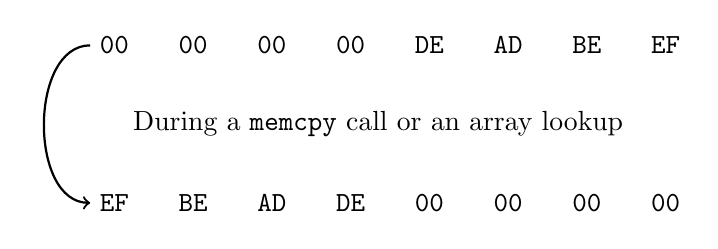
\begin{tikzpicture}
        \node (0)              {\texttt{00}};
        \node (1) [right of=0] {\texttt{00}};
        \node (2) [right of=1] {\texttt{00}};
        \node (3) [right of=2] {\texttt{00}};
        \node (4) [right of=3] {\texttt{DE}};
        \node (5) [right of=4] {\texttt{AD}};
        \node (6) [right of=5] {\texttt{BE}};
        \node (7) [right of=6] {\texttt{EF}};

        \node (H0) [below of=0] {};

        \node (A) [below of=H0]  {\texttt{EF}};
        \node (B) [right of=A] {\texttt{BE}};
        \node (C) [right of=B] {\texttt{AD}};
        \node (D) [right of=C] {\texttt{DE}};
        \node (E) [right of=D] {\texttt{00}};
        \node (F) [right of=E] {\texttt{00}};
        \node (G) [right of=F] {\texttt{00}};
        \node (H) [right of=G] {\texttt{00}};

        \draw [thick,out=180,in=180,->] (0) to node [right=1cm] {During a \texttt{memcpy} call or an array lookup} (A);
      \end{tikzpicture}
    \caption{The byte swap on a little-endian platform (i.e. C99 on \texttt{x86\_64})}
    \label{fig:little-endian}
  \end{figure}

The \texttt{Lyra2} class contains the main logic of the single-threaded Lyra2 instance. The functionality related to the sponge construction is captured by the \texttt{Sponge} \emph{abstract} class. Its subclasses \texttt{SpongeBlake2b}, \texttt{SpongeBlamka} and \texttt{SpongeHalfBlamka} hold the specifics of the underlying fixed-width permutation \(f\).

An insteresting detail is that the Sponge class in the Java project makes use of both left- and right bit rotations, done by the \texttt{rotl64} and \texttt{rotr64} methods respectively. The original Lyra2 reference implementation requires just one direction for rotations. Both types of rotations are helpful in the ported Java project because they allow to avoid a number of byte rotations related to endianness. For an example of this,  refer to figure \ref{fig:sponge-blake2b}. It shows the \texttt{SpongeBlake2b} implementation, where lines \(5, 8\), and \(11\) use a left rotation. This happens because the rotations there involve a whole number of bytes and there is no \texttt{mem.flip} call which performs an endianness-related rotation. On the contrary, line \(16\) expects a none-whole byte rotation (i.e. one bit rotation) which does not allow to repeat the same trick.


\begin{figure}
\small
\begin{minted}[linenos]{java}
    public class SpongeBlake2b extends Sponge {
        @Override
        public void G(final int a, final int b, final int c, final int d) {
            state[a] = mem.flip(mem.flip(state[a]) + mem.flip(state[b]));
            state[d] = rotl64(state[d] ^ state[a], 32);

            state[c] = mem.flip(mem.flip(state[c]) + mem.flip(state[d]));
            state[b] = rotl64(state[b] ^ state[c], 24);

            state[a] = mem.flip(mem.flip(state[a]) + mem.flip(state[b]));
            state[d] = rotl64(state[d] ^ state[a], 16);

            state[c] = mem.flip(mem.flip(state[c]) + mem.flip(state[d]));
            // Cannot use the left rotation trick here: 63 % 8 != 0, so
            // individual bytes do not stay the same, they change too.
            state[b] = mem.flip(rotr64(mem.flip(state[b] ^ state[c]), 63));
        }
    }
\end{minted}
\normalsize
\caption{Blake2b as instance of the Sponge class, illustrating optimized rotations}
\label{fig:sponge-blake2b}
\end{figure}

\chapter{Unit Testing Framework Choice}
\label{sec:unit-testing-framework-choice}

Chapter \ref{sec:unit-testing-framework-choice} discusses the choice of particular unit testing frameworks for the \texttt{lyra2-java} project. For an introduction to unit testing terms and basic practices please consult Section \ref{sec:unit-testing-fundamentals}. In this chapter, however, Section \ref{sec:unit-boost-google} discusses how two similar projects, the \texttt{lyra2-c} project and Argon2, address testing. Section \ref{sec:unit-junit-testng} and Section \ref{sec:unit-pytest} motivate the choice of tools and techniques for the \texttt{lyra2-java} project and the Python build harness.

Although the \texttt{lyra2-c} project has automated tests, it does not use a dedicated unit testing framework \cite{github:2017:lyra}. This is a justifiable choice which has its advantages. In particular, it allows to keep the complexity of the project under control and not rely on external libraries. The build process is somewhat simplified as well. Furthermore, when it comes to the C/C++ ecosystem, the choice of the framework is not trivial. The authors of Argon2 have also faced this choice and opted out to write their own test harness \cite{github:2017:argon2-test.c}. Section \ref{sec:unit-boost-google} will provide a plausible explanation for this decision.

\begin{table}
\begin{tabular}{llll}
    Name & License & Parametrization & Parallelism \\ \hline
Boost.Test & Boost Software License & yes & needs 3\textsuperscript{rd} party runner (\texttt{cmake}) \\
JUnit & Eclipse Public License & yes & needs 3\textsuperscript{rd} party runner (\texttt{mvn}) \\
py.test & MIT & yes & needs 3\textsuperscript{rd} party plugin (\texttt{xdist})
% Google Test & MIT & parameters? & yes
\end{tabular}
\caption{Important Features of Several Unit Testing Frameworks}
\label{table:framework-features-cpp}
\end{table}

\section{Boost.Test}
\label{sec:unit-boost-google}

There is a large choice of unit testing frameworks for the C/C++ ecosystem \cite{github:2017:google-test, github:2017:catch, boost:2017:test-docs}. Given the number of available solutions, their comparison and an educated choice would be a large and daunting task for any developer. This could be one of the reasons why project authors sometimes avoid using a unit testing framework altogether. Instead, they often write a separate test file that runs a few sanity checks.

For example, Argon2 uses its own \texttt{src/test.c} test program which was introduced on 25\textsuperscript{th} of January 2016 \cite{github:2017:argon2}. The commit hash starts with \texttt{7450df88} and it is number 317 out of (current) almost 600 in the version control history. This shows that this testing was introduced at the later stages of the project when the need for it was apparent \cite{github:2017:argon2-issue-85}.

A similar story could be observed for the reference Lyra2 project \cite{github:2017:lyra}. The rest of this section will attempt to demonstrate why a rather popular unit testing library Boost.Test was not used in either of the projects. This particular library was tried because of the personal developer preference of the author of this paper. A different developer could attempt the same steps with another library, like Catch \cite{github:2017:catch} or Google Test \cite{github:2017:google-test}.

Boost itself is a large collection of different libraries for C++ \cite{boost:2017:homepage}. It was originally founded by Dawes and Abrahams but today the number of contributors is in the hundreds. The scope of the libraries spans from concurrent programming to regular expressions to linear algebra. There is a formal submission process for any library that would like to be included into the collection \cite{boost:2017:submission-process} as well as rigorous review in the mailing lists \cite{boost:2017:mailing-list}.

The Boost.Test is a unit testing framework which is part of Boost \cite{boost:2017:test-docs}. It is licensed under the Boost Software License which is a free software license, approved by the Open Source Initiative and compatible with the \gls{gpl}. The library documentation can be found online \cite{boost:2017:test-docs}.

The main features of the library are summarized in \autoref{table:framework-features-cpp}. When it comes to password hashing, support for test parametrization becomes important because of the common test scenario described in Section \ref{sec:software-compatibility}. Boost.Test provides parametrization as well as other more common features of a unit testing library. In particular, the tests can be completely decoupled from the implementation, subdivided  into test suits and automatically registered with the test runner. The registration can be accomplished with a single \texttt{\#include<...>} and a call to the \texttt{BOOST\_AUTO\_TEST\_CASE} macro, as shown in \autoref{fig:boost-auto-test-case}.

\begin{listing}
\centering
\begin{minted}{cpp}
#define BOOST_TEST_MODULE example_module_name
#include <boost/test/included/unit_test.hpp>

BOOST_AUTO_TEST_CASE(name_of_test_function) {
    BOOST_TEST(true);
}
  \end{minted}
  \caption{Automatic Unit Test Registration With Boost.Test}
  \label{fig:boost-auto-test-case}
\end{listing}

Apart from that Boost.Test has a few convenience features. First of all, it was designed to be used as a header-only library. This means that the build process of a project needs only slight modification. Secondly, Boost.Test supports parametrized tests which are called "Data-driven Test Cases" and can be found in the documentation \cite{boost:2017:test-data-driven}. First step is to declare such tests with the special \texttt{BOOST\_DATA\_TEST\_CASE} macro. This macro informs the test runner that the corresponding test case requires test data in order to function. The data must be wrapped into a dataset in order to be passed into the test case, as described in the documentation \cite{boost:2017:test-docs-dataset}.

Password hashing algorithms often require several parameters in order to run, i.e. at least a password and a salt. In the case of Boost.Test it means that datasets must be somehow combined and manipulated together. For that reason operations such as \emph{joins}, \emph{zips} and \emph{grids} are supported by the dataset wrapper \cite{boost:2017:test-docs-dataset-operations}.

In conclusion, Boost.Test requires considerable setup in order to provide parametrized testing for password hashing algorithms. Although the documentation offers an accurate description of the process, it still takes significant effort and time to configure the test harness. The \texttt{lyra2-c} project and Argon2 understandably avoid these development costs by using their own unit testing programs.

\section{JUnit and TestNG}
\label{sec:unit-junit-testng}

The Java ecosystem offers a unit testing framework called JUnit \cite{junit:2017:homepage}. The basic components of this framework are described below.

The main element of JUnit is a \emph{test case} which is usually a class that contains testing logic. Such a class might have special methods called \emph{fixtures} which are responsible for setting up and tearing down the context in which a test is executed. For example, this might include repeatedly creating a set of objects or opening a database connection. The methods marked with the \texttt{@Before} (respectively, \texttt{@After}) annotation are executed before (respectively, after) each individual test. The \texttt{@BeforeClass} (respectively, \texttt{@AfterClass}) annotation ensures that a method is run exactly once before (respectively, after) the test class is instantiated.

Several test cases can be collected into a single \emph{test suite}. Finally, a program called a \emph{test runner} is responsible for discovering the test cases, running them and reporting the results back to the user. The test runner can be instructed to run (or skip) specific test suits.

In addition to JUnit, the Java ecosystem has a unit testing framework called TestNG \cite{testng:2017:home}. Below is a short comparison of the functionality relevant to testing password hashing algorithms.

Firstly, both frameworks offer parametrization tests but the implementation details are different. In order for a class to implement parametrized testing with JUnit4, it must be marked with the \texttt{@RunWith} annotation. That annotation must specify \texttt{Parameterized.class} as the test runner for the class. As well as that, the class must provide a method marked with the \texttt{@Parameters} annotation. This method should return a single \texttt{Collections<Object[]>} collection of test data \cite{junit:2017:parametrized-testing}. On the other hand, TestNG has two distinct mechanisms, one of which uses the \texttt{testng.xml} file and the other relies on a method with the \texttt{@DataProvider} annotation. In the second case the method should return either a single \texttt{Object[][]} array of test data or an \texttt{Iterator<Object[]>} iterator over such an array. With the first mechanism, the test data is stored directly in the \texttt{testng.xml} file. So, only the second approach allows to generate test data while  the tests are being run \cite{testng:2017:parametrized-testing}.

Based on the comparison above, the \texttt{lyra2-java} project was developed with JUnit4. There is nothing that would prohibit the usage of the TestNG framework for the same task. However, JUnit4 offers a single approach to writing parametrized unit tests which is flexible enough and does not make the developer choose between the different methods and different return values, as TestNG does. Finally, JUnit4 is often provided by default in modern Java development environments and does not require additional setup. Such availability has also played a major part in the choice of the unit testing framework for the \texttt{lyra2-java} project.

\begin{listing}
\small
\begin{minted}[linenos]{java}
@RunWith(Parameterized.class)
public class Lyra2Test {
    @Parameterized.Parameters
    public static Collection<Object[]> setupClass() {
        // Simplified initialization of a YAML data loader
        Yaml yaml = new Yaml();

        // A list of YAML file names with test vectors and resulting hashes
        String[] fnames = new String[] {"test-data-file_0.yml"};
        List<Object[]> entries = new ArrayList<>();

        for (String fname: fnames) {
            // Simplified loading of the YAML data from the file
            for (Object data : yaml.loadAll(reader)) {
                entries.add(new Object[]{data});
            }
        }

        return entries; // data provider has finished, returning result
    }

    private DataEntry entry;

    // Injection of test parameters
    public Lyra2Test(DataEntry entry) {
        this.entry = entry;
    }

    @Test
    public void simpleTest() {

        LyraParams params = new LyraParams(/* use entry to initialize */);

        byte[] hash = new byte[entry.klen];
        byte[] pass = entry.pass.getBytes();
        byte[] salt = entry.salt.getBytes();

        // Run the computation
        Lyra2.phs(hash, pass, salt, params);
        // Fetch the correct hash value
        byte[] correct_hash = pack.bytes(entry.hash);
        // Compare the computation result to the correct hash
        assertArrayEquals(correct_hash, hash);
    }
}
\end{minted}
\normalsize
\caption{Example of JUnit4 Parametrized Testing for the \texttt{lyra2-java} Project}
\label{fig:junit4-parametrization}
\end{listing}

\autoref{fig:junit4-parametrization} provides a simplified example of the way unit tests are organized in the \texttt{lyra2-java} project. The testing logic is in the \texttt{simpleTest} method: configuration parameters are constructed using the values from the \texttt{entry} instance variable, then a call to the \texttt{Lyra2.phs} method is made to compute the hash. The result of the computation is then compared to the correct answer by the call to the \texttt{assertArrayEquals} method.

The \texttt{setupClass} method is marked with the \texttt{@Parametrized.Parameters} annotation which makes this method the provider of data. The precomputed data comes from several \gls{yaml} data files whose names are stored in the \texttt{fnames} variable. More information about the \gls{yaml} format in general and the test data file structure in particular can be found in Section \ref{sec:configuration-and-test-file-format}. The \texttt{for} loop on line 12 sequentially opens the \gls{yaml} data files, loads their contents and collects them in the \texttt{entries} collection variable. Once the \texttt{setupClass} method returns that variable, it is used by JUnit to initialize several instances of the class, providing each constructor with one set of test data from the \texttt{entries} collection.

This is the application of the parametrized testing approach which allows to run several hundreds of tests for different configurations and input values while writing the logic for the testing code only once.

\section{Unit Testing With py.test}
\label{sec:unit-pytest}

Python is a popular high-level general purpose scripting language created by van Rossum \cite{python:2017:homepage}. It has a built-in unit testing framework called unittest \cite{python:2017:unittest-homepage} which comes together with the interpreter. Similar to JUnit4, it expects the developer to provide a hierachy of test classes grouped into test modules. Other two notable unit testing frameworks in the Python ecosystem are Nose \cite{nose:2017:homepage} and py.test \cite{pytest:2017:homepage}. They are both similar to the built-in unittest framework but at the same time offer more flexibility: the developer does not \emph{have to} organize their tests into classes, parametrized testing is readily available and parallelized test execution can be taken advantage of as well.

The design of the unittest framework does not offer a dedicated mechanism to write parametrized tests. At the same time the Nose library implements parametrized testing by making use of Python generators (the \texttt{yield} keyword). They generate separate functions at runtime which are then executed as standalone test cases \cite{nose:2017:parametrized-testing}. On the other hand, the py.test framework does not use Python generators but instead relies on the \texttt{@mark.parametrized} decorator \cite{pytest:2017:parametrized-testing}. A usage example can be found in \autoref{fig:pytest-parametrization}.

Unfortunately, the Nose unit testing framework is currently in maintenance mode. This framework is no longer in active development and therefore is not recommended for new projects. This is why the Python build harness for the \texttt{lyra2-c} project uses the py.test framework.

\begin{listing}
\begin{minted}[linenos]{python}
import pytest
import subprocess

from pathlib import Path

bindir = Path(__file__).parent.parent.joinpath('bin42')
@pytest.mark.parametrize('path', list(bindir.glob("lyra2-*")))
@pytest.mark.parametrize('pwd', ['password', 'qwerty'])
@pytest.mark.parametrize('salt', ['salt', 'pepper'])
@pytest.mark.parametrize('k', [1, 2])
@pytest.mark.parametrize('t', [1, 2])
@pytest.mark.parametrize('m', [3, 4, 5, 6, 7, 8, 9, 10])
def test_sanity_0(path, pwd, salt, k, t, m):

    result = subprocess.run([path, pwd, salt, str(k), str(t), str(m)])

    assert result.returncode == 0
\end{minted}
\caption{Simplified Example of py.test Parametrized Testing for Python Build Harness}
\label{fig:pytest-parametrization}
\end{listing}

\autoref{fig:pytest-parametrization} shows why parametrized testing is important when building different configurations of the reference Lyra2 implementation. Before running those configurations it is reasonable to make sure that the compiled executable files actually work. However, since there are many parameters that can be configured at compile time (such as the number of columns or the size of the block of the memory matrix), writing a test for each individual possible configuration is not feasible. Instead, each generated executable file is prefixed with \texttt{lyra2-} and has other compile time parameters listed in the filename, like the aforementioned number of columns or size of the block. Then the \texttt{@pytest.mark.parametrize('path')} decorator is used to fetch all the matching filenames from the build directory. Each of these names is later used as the \texttt{path} parameter to create the corresponding unit test case dynamically.

This parametrized testing approach allows to write the testing logic once and reuse it for any possible Lyra2 configuration produced by the \texttt{Makefile} of the reference project.

%%%%%%%%%%%%%%%%%%%%%%%%%%%%%%%%%%%%%%%%%%%%%%%%%%%%%%%%%%%%%%%%%%%%%%%%
\section{Configuration and Test File Format}
%%%%%%%%%%%%%%%%%%%%%%%%%%%%%%%%%%%%%%%%%%%%%%%%%%%%%%%%%%%%%%%%%%%%%%%%
\label{sec:configuration-and-test-file-format}

The data for parametrized tests is stored in \gls{yaml} files. Those files are produced by the \texttt{lyra2-c} project with the help of the Python build harness. Then they are consumed by the JUnit testing framework of the \texttt{lyra2-java} project. This mechanism allows to make sure that both projects compute the same hash values.

YAML stands for \emph{YAML Ain't Markup Language} and is a superset of \gls{json}, another popular data format. \gls{yaml} targets human readability and provides native support for custom datatypes: scalars, arrays, structures, etc. \cite{yaml:2017:specification}. Most programming languages provide support for reading and writing of \gls{yaml} files, including both Java and Python.

A single file in \gls{yaml} can hold several documents. This feature is leveraged by the Python build harness. In particular, each \gls{yaml} file corresponds to a single Lyra2 executable. This guarantees that exactly one Lyra2 executable is used to compute the test data hashes from that file. So, the compile time parameters are the same for the contents from that file. These parameters are stored together with all the runtime parameters and the resulting hash, see \autoref{fig:yaml-data} for reference. The \texttt{hash} field is stored as an array of strings which ensures that different \gls{yaml} libraries deduce the content type of this array correctly. The \texttt{-{}-{}-} is a delimiter between the two \gls{yaml} documents.

The \gls{yaml} format is also used to store default configuration for the Python build harness of the reference Lyra2 project. It can be found in the \texttt{harness} branch of the forked reference repository in the \texttt{harness.yml} file \cite{github:2017:lyra-copy}. The primary parameters are \texttt{build\_path} and \texttt{makefile\_path}. The first one defines the location for the compiled Lyra2 executable files and the second one points to the original \texttt{Makefile}.

The \texttt{matrix} group of parameters defines the build matrix. The \texttt{option} parameter configures the type of Lyra2 executable built by the \texttt{Makefile}, which is a generic version for the \texttt{x86\_64} architecture by default. The \texttt{threads} parameter determines the parallelism degree and is set to 1. The \texttt{columns}, \texttt{sponge}, \texttt{rounds} and \texttt{blocks} correspond directly to compile time Lyra2 parameters. Finally, the \texttt{bench} parameter determines if the test vectors should be included into the compiled executable. By default it is set to 0 which means those vectors are skipped.

The \texttt{data} group of parameters specifies the test vectors which will be used when generating hash values with \texttt{./harness.py compute}. That group includes \texttt{pass}~---~an array of passwords, \texttt{salt}~---~an array of salts, \texttt{klen}~---~an array of output lengths (i.e. the length of the hash), \texttt{tcost}~---~an array of time costs and finally \texttt{mcost}~---~an array of memory costs. The \texttt{./harness.py} script generates a grid of all of the possible value combinations and then runs every compiled executable using those values as test data. The resulting hashes are stored in the \texttt{data\_path} directory which can be configured as well. The \texttt{./harness.py} script does not overwrite old hash values, so you must remove them manually if regeneration is required.

Finally, compilation flags are also part of the configuration and their defaults can be seen in \autoref{fig:compile-flags}.

\begin{listing}
    \begin{minted}{yaml}
    blocks: 8
    columns: 16
    hash: [0f, ee, bd, 1f, '00', 2a, 5b, '87', '71', ee]
    klen: 10
    mcost: 3
    pass: password
    rounds: 1
    salt: s
    sponge: blake2b
    tcost: 1
    threads: 1
    ---
    blocks: 8
    columns: 16
    hash: [0f, 7d, e3, 3c, e3, 9e, 0c, f9, 8e, '70']
    klen: 10
    mcost: 10
    pass: password
    rounds: 1
    salt: s
    sponge: blake2b
    tcost: 1
    threads: 1
    \end{minted}
    \caption{Example of a YAML Test Data File: distinct documents are separated with \mintinline{shell}{---}.}
    \label{fig:yaml-data}
\end{listing}


\begin{listing}
    \begin{minted}{yaml}
    CFLAGS:
      - -std=c99
      - -Wall
      - -pedantic
      - -O3
      - -msse2
      - -ftree-vectorizer-verbose=1
      - -fopenmp
      - -funroll-loops
      - -march=native
      - -Ofast
      - -mprefer-avx128
      - -flto
      \end{minted}
      \caption{Compilation Flags Used by the \texttt{lyra2-c} Project}
      \label{fig:compile-flags}
  \end{listing}

%%%%%%%%%%%%%%%%%%%%%%%%%%%%%%%%%%%%%%%%%%%%%%%%%%%%%%%%%%%%%%%%%%%%%%%%
\chapter{Results}
\label{sec:results}
%%%%%%%%%%%%%%%%%%%%%%%%%%%%%%%%%%%%%%%%%%%%%%%%%%%%%%%%%%%%%%%%%%%%%%%%

This chapter presents the main results of the porting effort. In particular, section \ref{sec:it-works} covers algorithm-level compatibility. Section \ref{sec:performance-comparison} compares performance of the reference and the ported implementations on a number of different configurations of the Lyra2 algorithm. Finally, section \ref{sec:mobile-application} demonstrates the ease of integration of the ported project into an Android mobile application.

\section{Algorithm-level Compatibility}
\label{sec:it-works}

The primary goal of this work was to port Lyra2 to Java so that it would produce the same hash values as the reference implementation when given the same inputs. Such algorithm-level compatibility was achieved and will be demonstrated in section \ref{sec:manual-testing} and section \ref{sec:automated-testing}. The former deals with hand-picked test vectors while the latter demonstrates a reasonably large collection of randomly picked test vectors and a unit-testing framework which uses them to verify hash results.

\subsection{Configuration Choice}
By design Lyra2 has a large number of configurable parameters. This section will provide the reasoning behind the choice of particular values. The short summary can be found in table \ref{table:configuration-summary}.

There are three sponges that could be tested: Blake2b, BlaMka and half-round BlaMka. Only the first two are in the manual testing shortlist because half-round BlaMka is similar to BlaMka. The sponge block size can be either 8, 10 or 12, so the extreme values made it into the shortlist. The columns of the memory matrix can be any positive number. The \path{Lyra2/src/runBenchCPU.sh} benchmarking script as well as other sources suggest that the values of 256 and 512 should be chosen.

Finally, time and memory costs are fixed at an arbitrary value of 100. The output length is chosen to be 10 so that the resulting hash value would fit easily on the page.

\begin{table}
\begin{center}
\begin{tabular}{l r}
Parameter & Value \\ \hline
Sponge & Blake2b, BlaMka \\
Sponge blocks & 8, 12 \\
Sponge rounds & 12 \\
Columns in the memory matrix & 256, 512 \\
Time cost (number of iterations) & 100 \\
Memory cost (number of rows in the memory matrix) & 100 \\
Output length (bytes) & 10 \\
\end{tabular}
\end{center}
\caption{Summary of parameter values for manually tested configurations}
\label{table:configuration-summary}
\end{table}

\subsection{Manual Testing}
\label{sec:manual-testing}

Figure \ref{fig:manual-testing} shows a log of manual tests. New line delimits different Lyra2 configurations. The first line of each group represents a particular configuration group: \verb|--outlen| is the output length, \verb|--tcost| is the time cost, \verb|--mcost| is the memory cost. The second and the forth line in each group is the password and salt pair, and the third and fifth lines are the resulting hash values.

\begin{figure}[p]
\begin{minted}[fontsize=\footnotesize]{shell}
$ lyra2 --sponge blake2b --blocks 8 --columns 256 --outlen 10 --tcost 100 --mcost 100
> "password" "salt"
> 19 FD 3B 50 9A 03 0C DF 95 DA
> "The quick brown fox jumped over the lazy dog" "0123456789"
> 04 A0 BF 30 D1 E5 A5 05 53 E9

$ lyra2 --sponge blake2b --blocks 8 --columns 512 --outlen 10 --tcost 100 --mcost 100
> "password" "salt"
> 73 39 79 B6 C1 3C C1 F3 D7 17
> "The quick brown fox jumped over the lazy dog" "0123456789"
> A1 B0 18 F6 B6 79 5F E0 2A A4

$ lyra2 --sponge blake2b --blocks 12 --columns 256 --outlen 10 --tcost 100 --mcost 100
> "password" "salt"
> 9C 52 2A B9 18 30 F9 E7 09 55
> "The quick brown fox jumped over the lazy dog" "0123456789"
> 7D B2 9D C8 31 B4 E9 0E 10 22

$ lyra2 --sponge blake2b --blocks 12 --columns 512 --outlen 10 --tcost 100 --mcost 100
> "password" "salt"
> AC F2 B6 50 2D BC F0 62 DD 29
> "The quick brown fox jumped over the lazy dog" "0123456789"
> 4F 1B 03 6B C9 A2 09 C4 BC DA

$ lyra2 --sponge blamka --blocks 8 --columns 256 --outlen 10 --tcost 100 --mcost 100
> "password" "salt"
> 53 32 F3 D7 C4 9C 46 38 3C 1B
> "The quick brown fox jumped over the lazy dog" "0123456789"
> E7 6E 4B A0 81 B8 3C CF D6 64

$ lyra2 --sponge blamka --blocks 8 --columns 512 --outlen 10 --tcost 100 --mcost 100
> "password" "salt"
> D9 F9 F5 65 0D 05 88 D0 DF F6
> "The quick brown fox jumped over the lazy dog" "0123456789"
> 3A 3D 40 00 3E 33 44 45 B3 DD

$ lyra2 --sponge blamka --blocks 12 --columns 256 --outlen 10 --tcost 100 --mcost 100
> "password" "salt"
> C1 BC 48 80 99 1C E7 E6 52 18
> "The quick brown fox jumped over the lazy dog" "0123456789"
> 2E 4E 56 C7 5B 3D B7 F9 E0 30

$ lyra2 --sponge blamka --blocks 12 --columns 512 --outlen 10 --tcost 100 --mcost 100
> "password" "salt"
> 82 AF EB 03 5B E7 12 11 BE 63
> "The quick brown fox jumped over the lazy dog" "0123456789"
> F7 A8 56 D5 81 16 AA E5 C7 4D
\end{minted}
\caption{Manual testing protocol, each configuration starts with \texttt{\$}, each password and salt pair is followed by the resulting hash value. The hash value is printed in hexadecimal.}
\label{fig:manual-testing}
\end{figure}

\subsection{Automated Testing}
\label{sec:automated-testing}

The automated testing is possible because of the additional code that was added to the reference implementation. As mentioned in section \ref{sec:reference-implementation}, there is a \verb|harness| branch which could be found in the forked GitHub project \cite{github:2017:lyra-copy} and the corresponding pull request \cite{github:2017:lyra-pr}. This branch introduces the \verb|Lyra2/tests/harness.py| script written in Python 3 which allows to compile several configurations of Lyra2 and then use those to compute and store hash values.

Additionally, the \verb|Lyra2/tests/take.py| Python 3 script was used to choose a number of random hash values from those previously precomputed. These were then used in the Java project to unit-test the implementation. Some of the hash values were also included into the continuous integration service and their status can be verified by visiting \cite{travis:2017:lyra}. However, continuous integration runs only a subset of the vectors that were run locally due to the limited amount of memory available on the remote machines. In conclusion, both manual and automated testing indicate that the ported implementation does not contain immediately visible problems.

\section{Performance Comparison}
\label{sec:performance-comparison}

The single-threaded configuration of the reference C implementation was compared to its ported Java counterpart. For that, a separate GitHub repository was set up in \cite{github:2017:lyra2-compare}. This repository needs to control software written in both C and Java which is why an expressive, high-level scripting language was chosen to complete this task: Python 3.

\subsection{Project Structure}

The comparison project \cite{github:2017:lyra2-compare} is a combination of two Jupyter Notebooks \cite{jupyter:2017:jupyter} and an SQlite database. The two created notebooks follow the producer-consumer strategy. The \mintinline{shell}{src/compare.ipynb} is the producer notebook which is responsible for compiling both C and Java implementations as well as dispatching computation tasks. The results are then collected into the \mintinline{shell}{measurements.db} SQLite database (which also serves as a cache layer). The consumer is the \mintinline{shell}{src/plot.ipynb} notebook which reads the data from the SQLite database and plots the figures shown below.

Lyra2 provides two main adjustable parameters: time and memory cost. Changing both of the parameters at the same time cannot be easily shown on a single graph which is why the comparison contains three main parts. Subsections \ref{sec:fixed-time-cost} and \ref{sec:fixed-memory-cost} show how several Lyra2 configurations behave when time cost and memory cost is fixed, respectively. Subsection \ref{sec:no-fixed-costs} shows a grid of values for both time and memory costs. In all the sections, the two projects are compared using four configurations:

\begin{itemize}
    \item Blake2b sponge with 256 columns, figures \ref{figure:mcost_256}, \ref{figure:tcost_256} and \ref{figure:tcost_mcost_blake2b_256}
    \item Blake2b sponge with 2048 columns, figures \ref{figure:mcost_2048}, \ref{figure:tcost_2048} and \ref{figure:tcost_mcost_blake2b_2048}
    \item BlaMka sponge with 256 columns, figures \ref{figure:mcost_256}, \ref{figure:tcost_256} and \ref{figure:tcost_mcost_blamka_256}
    \item BlaMka sponge with 2048 columns, figures \ref{figure:mcost_2048}, \ref{figure:tcost_2048} and \ref{figure:tcost_mcost_blamka_2048}
  \end{itemize}

Configurations were run in parallel, creating one process per configuration. Running time was measured as the time between process creation and its termination. Memory consumption was recorded from the parent process and its peak value was stored. For more details, please consult the \texttt{src/compare.ipynb} and \texttt{src/plot.ipynb} notebooks from \cite{github:2017:lyra2-compare}.

Finally, in subsection \ref{sec:no-fixed-costs} the grid of time and memory cost parameters is \(200 \times 200\) with a step of \(10\), which results in a total of \(8 \times 21 \times 21 = 3528\) measurements used to build all the graphics.

\subsection{Fixed Time Cost}
\label{sec:fixed-time-cost}

There are two figures that show how running time and consumed memory depend on memory cost when time cost is fixed. Figure \ref{figure:mcost_256} shows a 256-column and figure \ref{figure:mcost_2048} shows a 2048-column configuration of Lyra2. Both these figures show that the reference implementation works faster and consumes less memory than its Java counterpart. A nice property is that both the running time and memory consumption are changing roughly linearly as the memory cost parameter is changed. This is consistent with the fact that the memory cost parameter corresponds to the number of rows of the in-memory matrix. There are some outliers with respect to both running time and memory consumption which can be attributed to different system loads.

\begin{figure}[H]
    \centering
    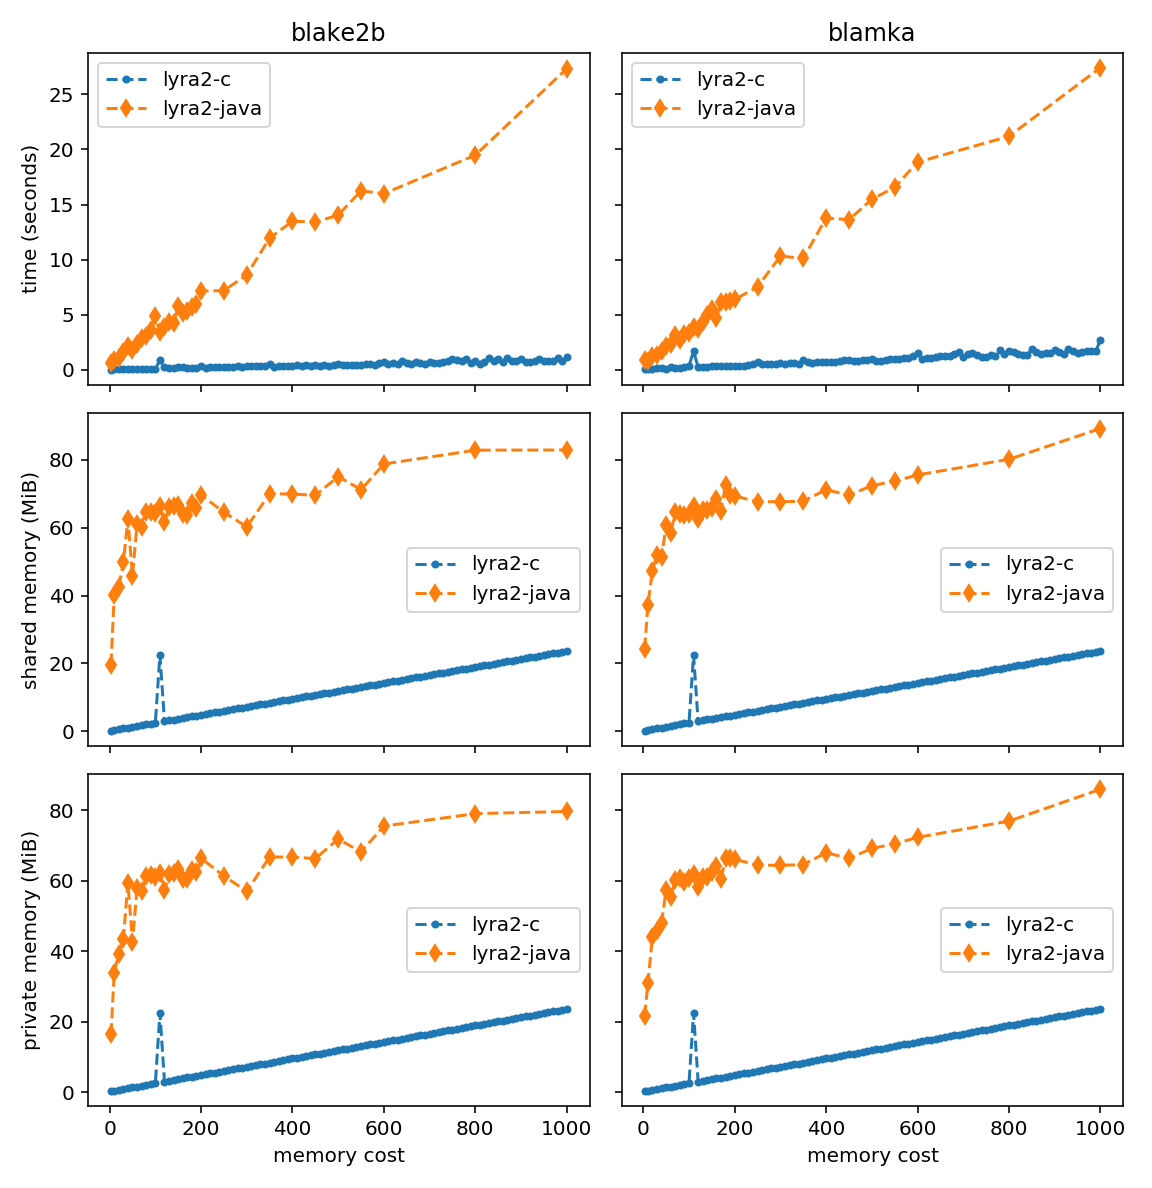
\includegraphics[width=\linewidth,keepaspectratio]{figures/mcost_256}
    \caption{\texttt{lyra2-c} compared to \texttt{lyra2-java}: 256 columns, fixed time cost of 10. Blake2b sponge on the left, BlaMka sponge on the right.}
    \label{figure:mcost_256}
\end{figure}

\begin{figure}[H]
    \centering
    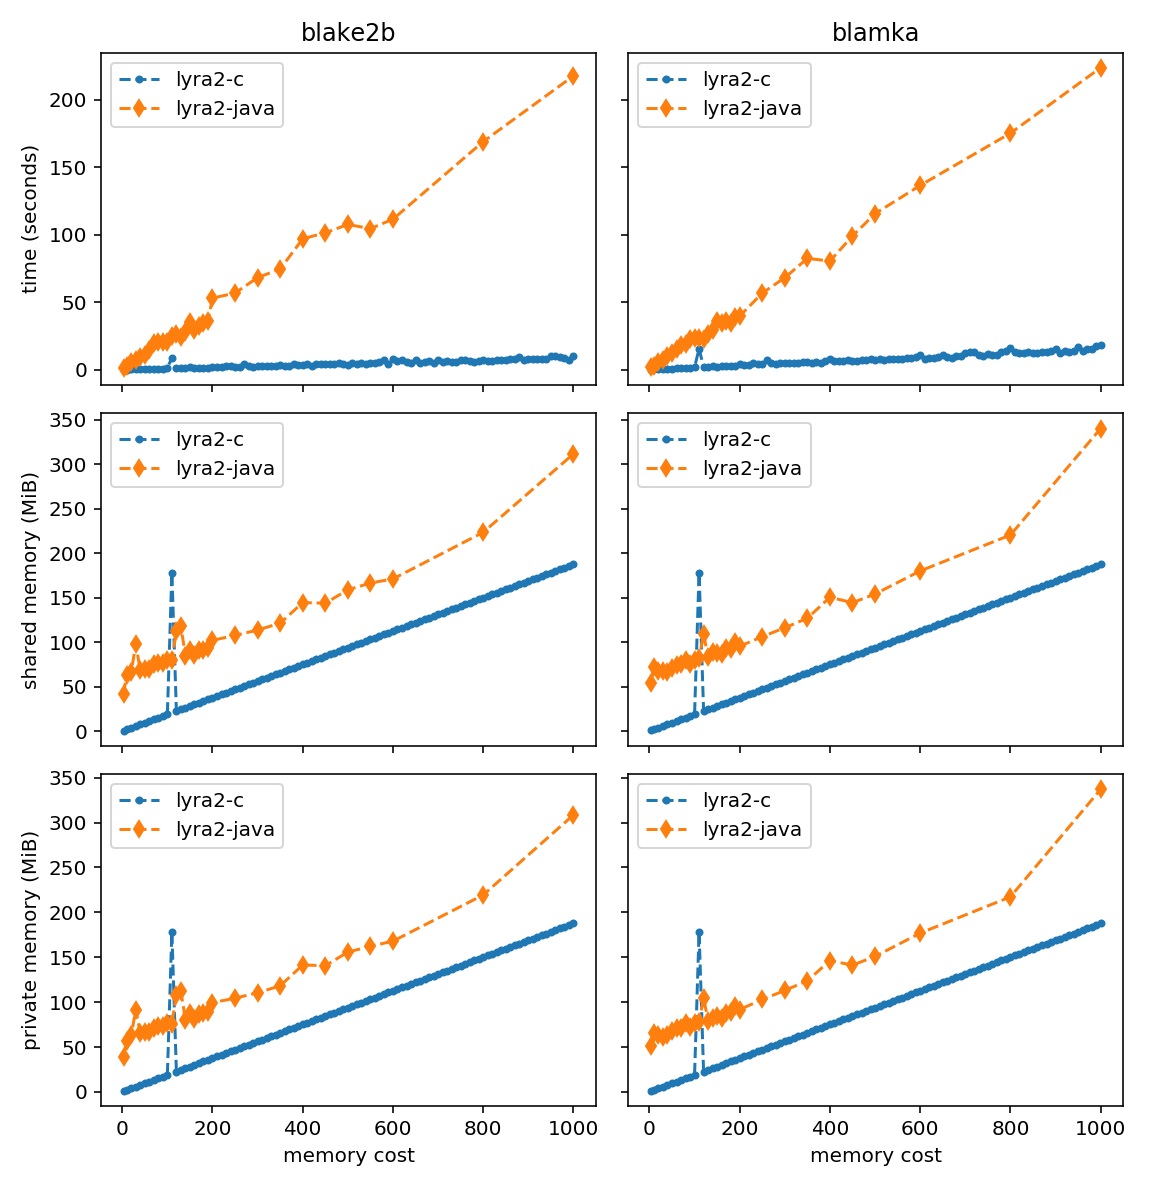
\includegraphics[width=\linewidth,keepaspectratio]{figures/mcost_2048}
    \caption{\texttt{lyra2-c} compared to \texttt{lyra2-java}: 2048 columns, fixed time cost of 10. Blake2b sponge on the left, BlaMka sponge on the right.}
    \label{figure:mcost_2048}
\end{figure}

\subsection{Fixed Memory Cost}
\label{sec:fixed-memory-cost}

There are two figures that show how running time and consumed memory depend on time cost when memory cost is fixed. Figure \ref{figure:tcost_256} shows a 256-column and figure \ref{figure:tcost_2048} shows a 2048-column configuration of Lyra2. Both these figures show that the original C implementation works faster and consumes less memory than its Java counterpart. The running time changes roughly linearly as the time cost parameter is changed which is consistent with the fact that time cost corresponds to the number of iterations done by Lyra2. Memory consumption stays roughly the same which is also consistent with the fact that the largest memory consumer is the in-memory matrix. This matrix has the same size for all of the configurations. Admittedly, there are some deviations in memory consumption of the Java implementation. The second set of figures \ref{figure:tcost_2048} even has a slight downward trend. The possible reasons for that include: the built-in garbage collector and the fact that the measurements run for several days, resulting in potentially different system loads.

\begin{figure}[H]
    \centering
    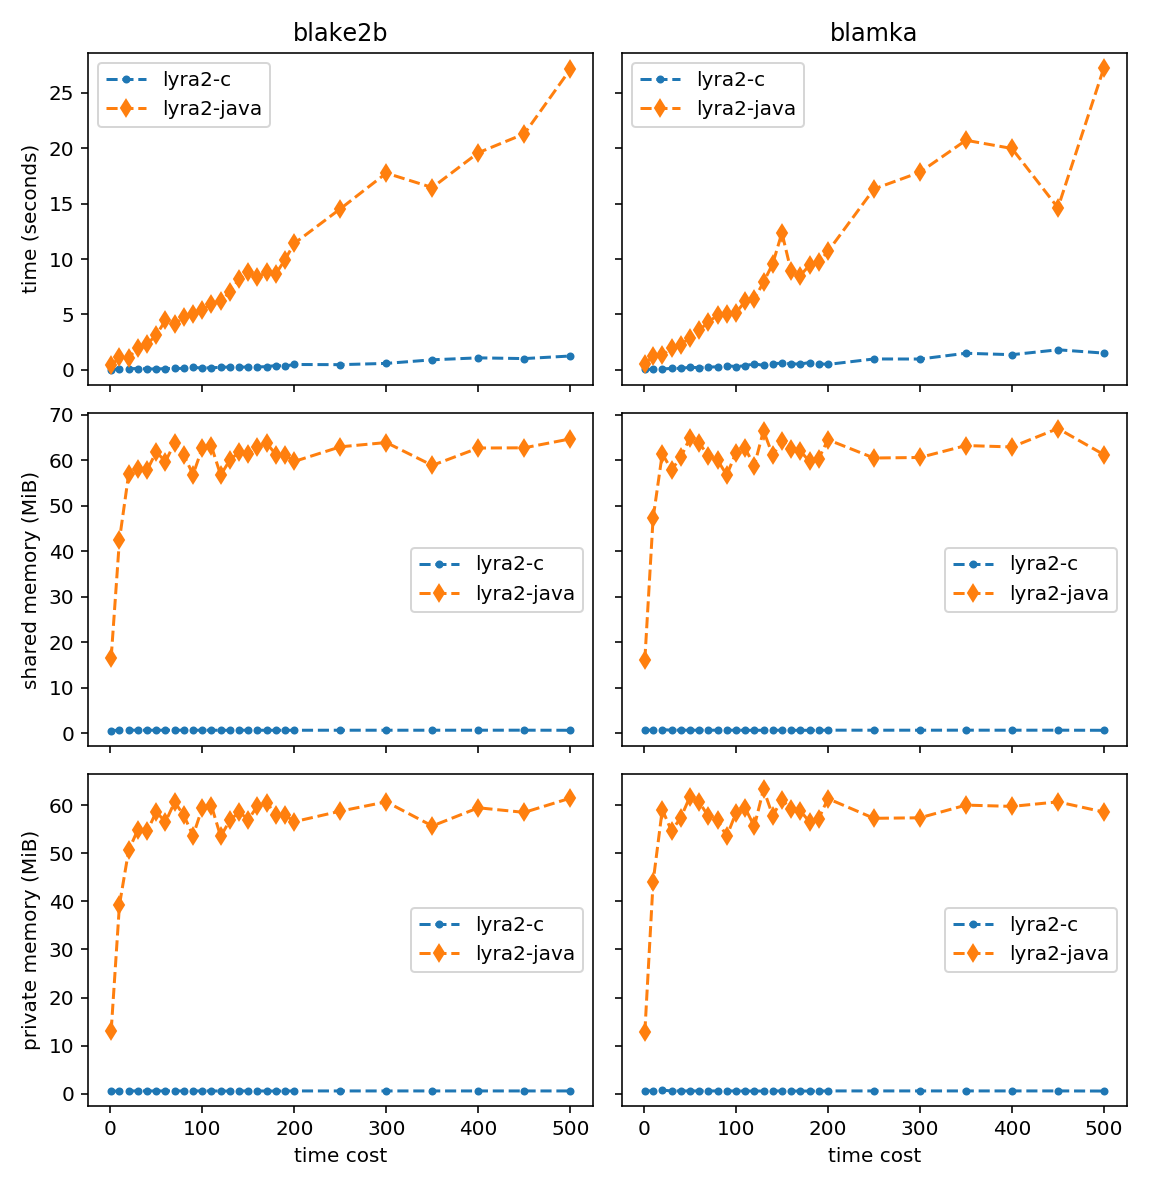
\includegraphics[width=\linewidth,keepaspectratio]{figures/tcost_256}
    \caption{\texttt{lyra2-c} compared to \texttt{lyra2-java}: 256 columns, fixed memory cost of 20. Blake2b sponge on the left, BlaMka sponge on the right.}
    \label{figure:tcost_256}
\end{figure}

\begin{figure}[H]
    \centering
    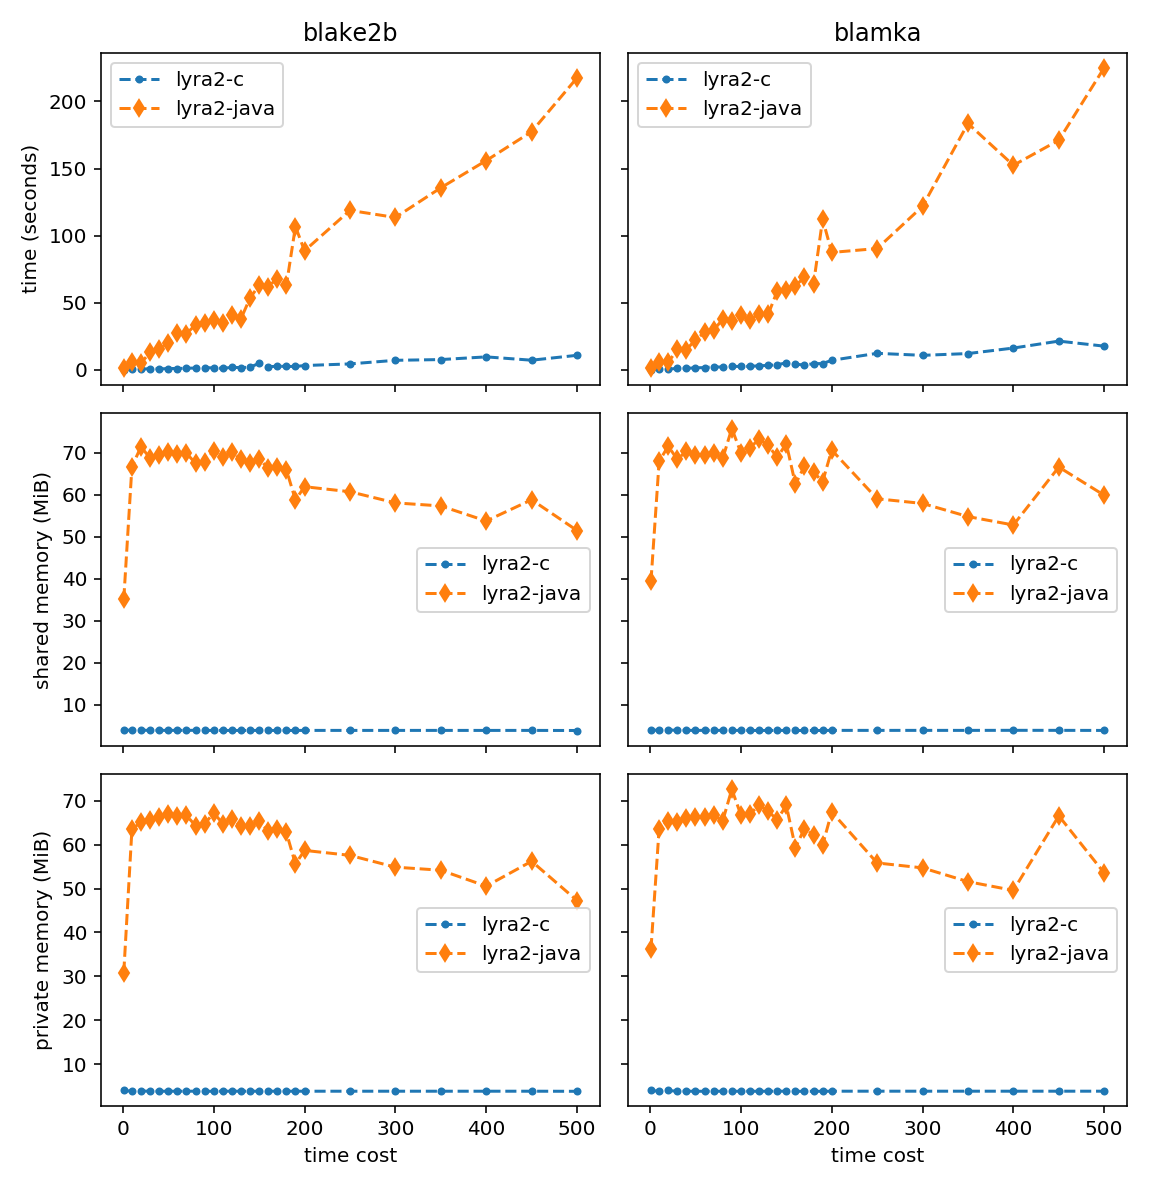
\includegraphics[width=\linewidth,keepaspectratio]{figures/tcost_2048}
    \caption{\texttt{lyra2-c} compared to \texttt{lyra2-java}: 2048 columns, fixed memory cost of 20. Blake2b sponge on the left, BlaMka sponge on the right.}
    \label{figure:tcost_2048}
\end{figure}

\subsection{Variable Time and Memory Costs}
\label{sec:no-fixed-costs}

There are four figures that show running time and memory consumption of Lyra2 when both time and memory costs change. Figures \ref{figure:tcost_mcost_blake2b_256} and \ref{figure:tcost_mcost_blake2b_2048} correspond to a 256- and 2048-column configurations of Lyra2 that both use the Blake2b sponge. Figures \ref{figure:tcost_mcost_blamka_256} and \ref{figure:tcost_mcost_blamka_2048} are the 256- and 2048-column configurations of Lyra2 with the BlaMka sponge. All of these four figures share the same properties. First of all, the reference implementation is faster and consumes less memory than its Java counterpart. Secondly, the running time as well as required space depend roughly linearly on the time and memory cost parameters. However, together they create a quadratic time growth during the \emph{Wandering phase}. This still allows for predictable and fine-tuned control of the time and memory resources required by the algorithm.

\begin{figure}[p]
    \centering
    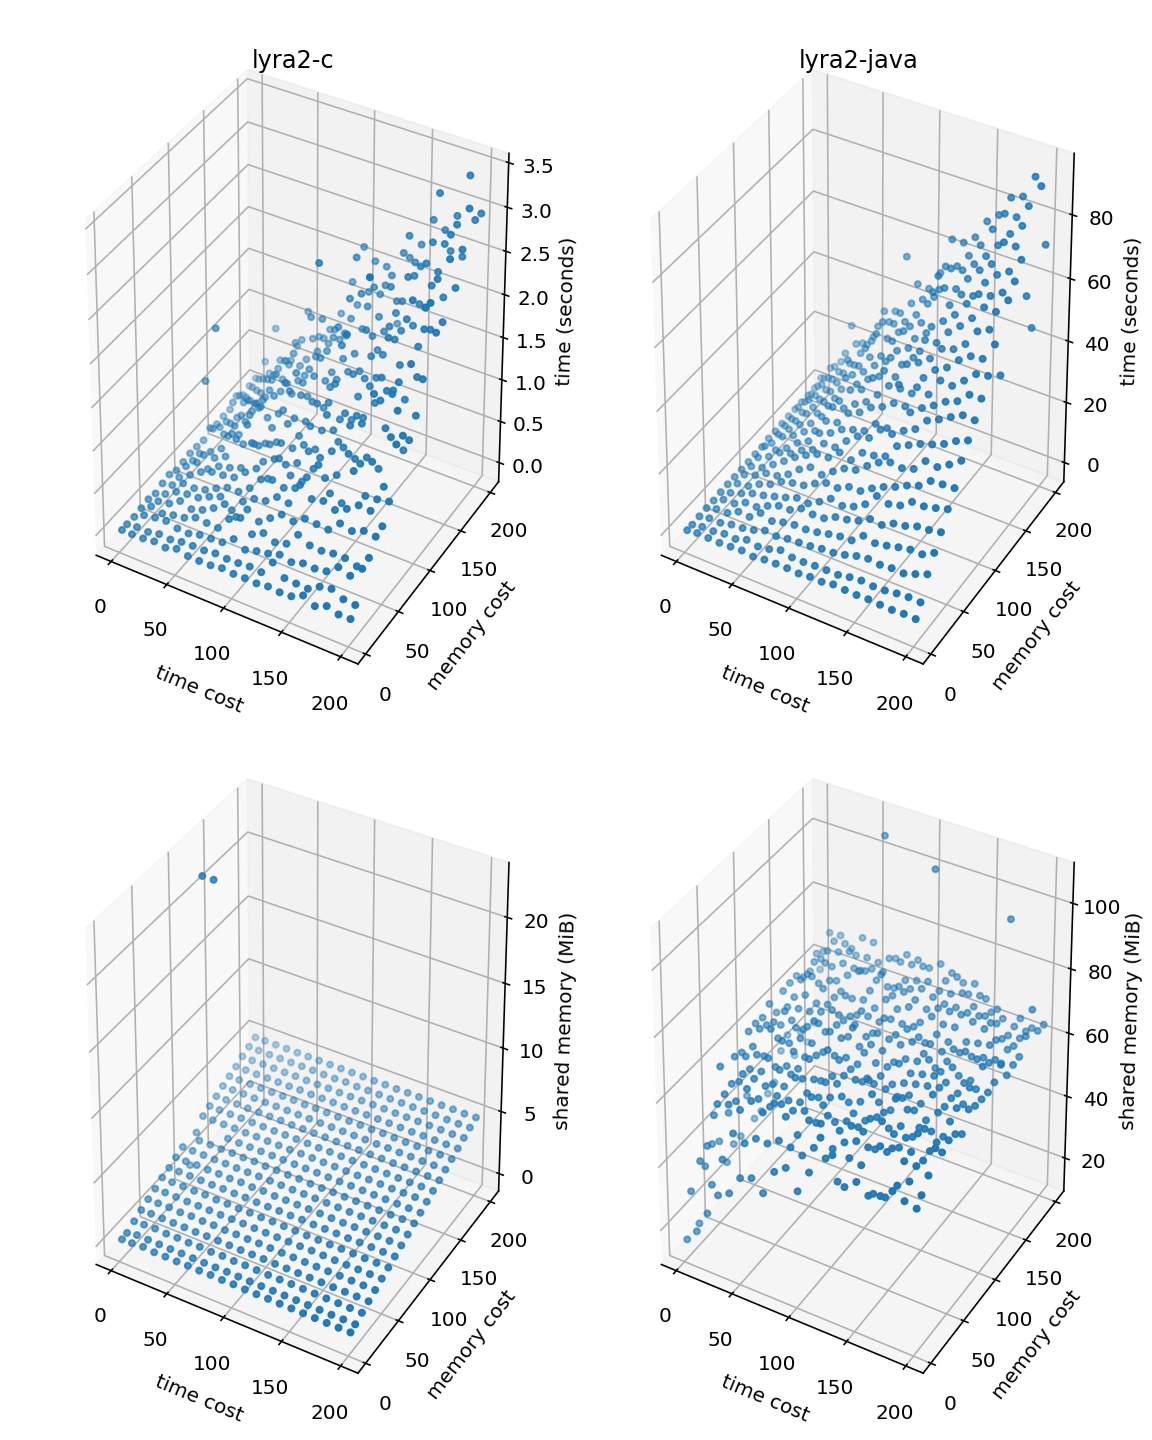
\includegraphics[width=\linewidth,keepaspectratio]{figures/tcost_mcost_blake2b_256}
    \caption{\texttt{lyra2-c} compared to \texttt{lyra2-java}: Blake2b sponge, 256 columns.}
    \label{figure:tcost_mcost_blake2b_256}
\end{figure}

\begin{figure}[p]
    \centering
    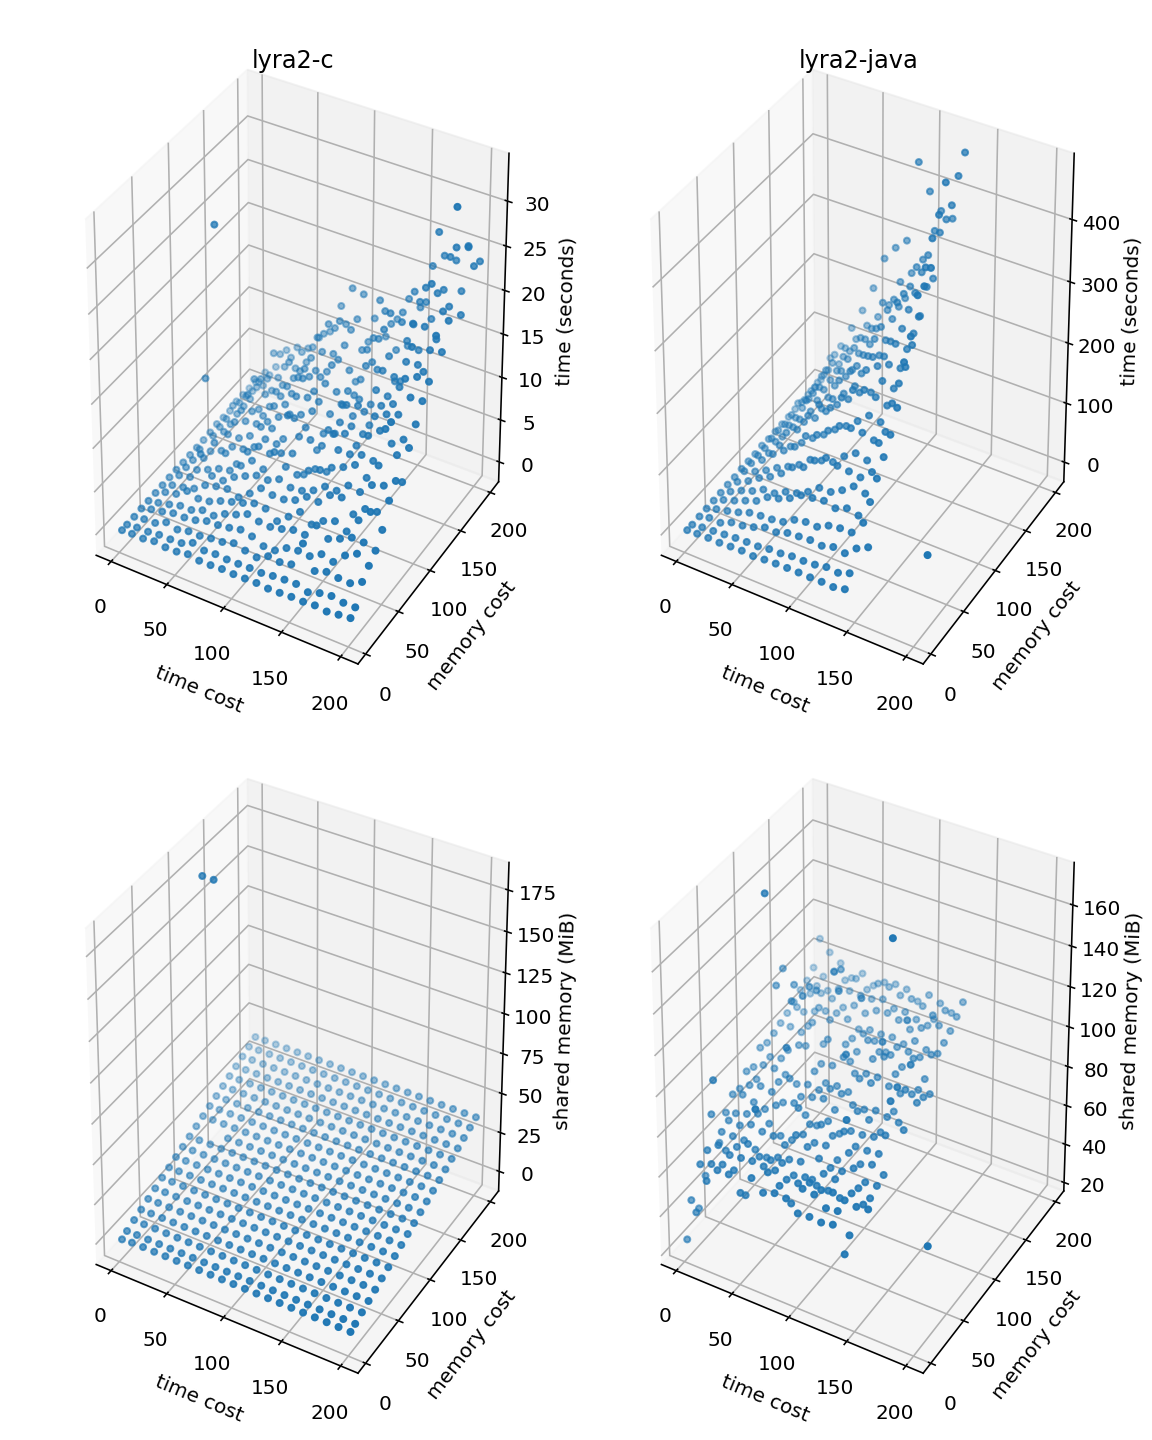
\includegraphics[width=\linewidth,keepaspectratio]{figures/tcost_mcost_blake2b_2048}
    \caption{\texttt{lyra2-c} compared to \texttt{lyra2-java}: Blake2b sponge, 2048 columns.}
    \label{figure:tcost_mcost_blake2b_2048}
\end{figure}

\begin{figure}[p]
    \centering
    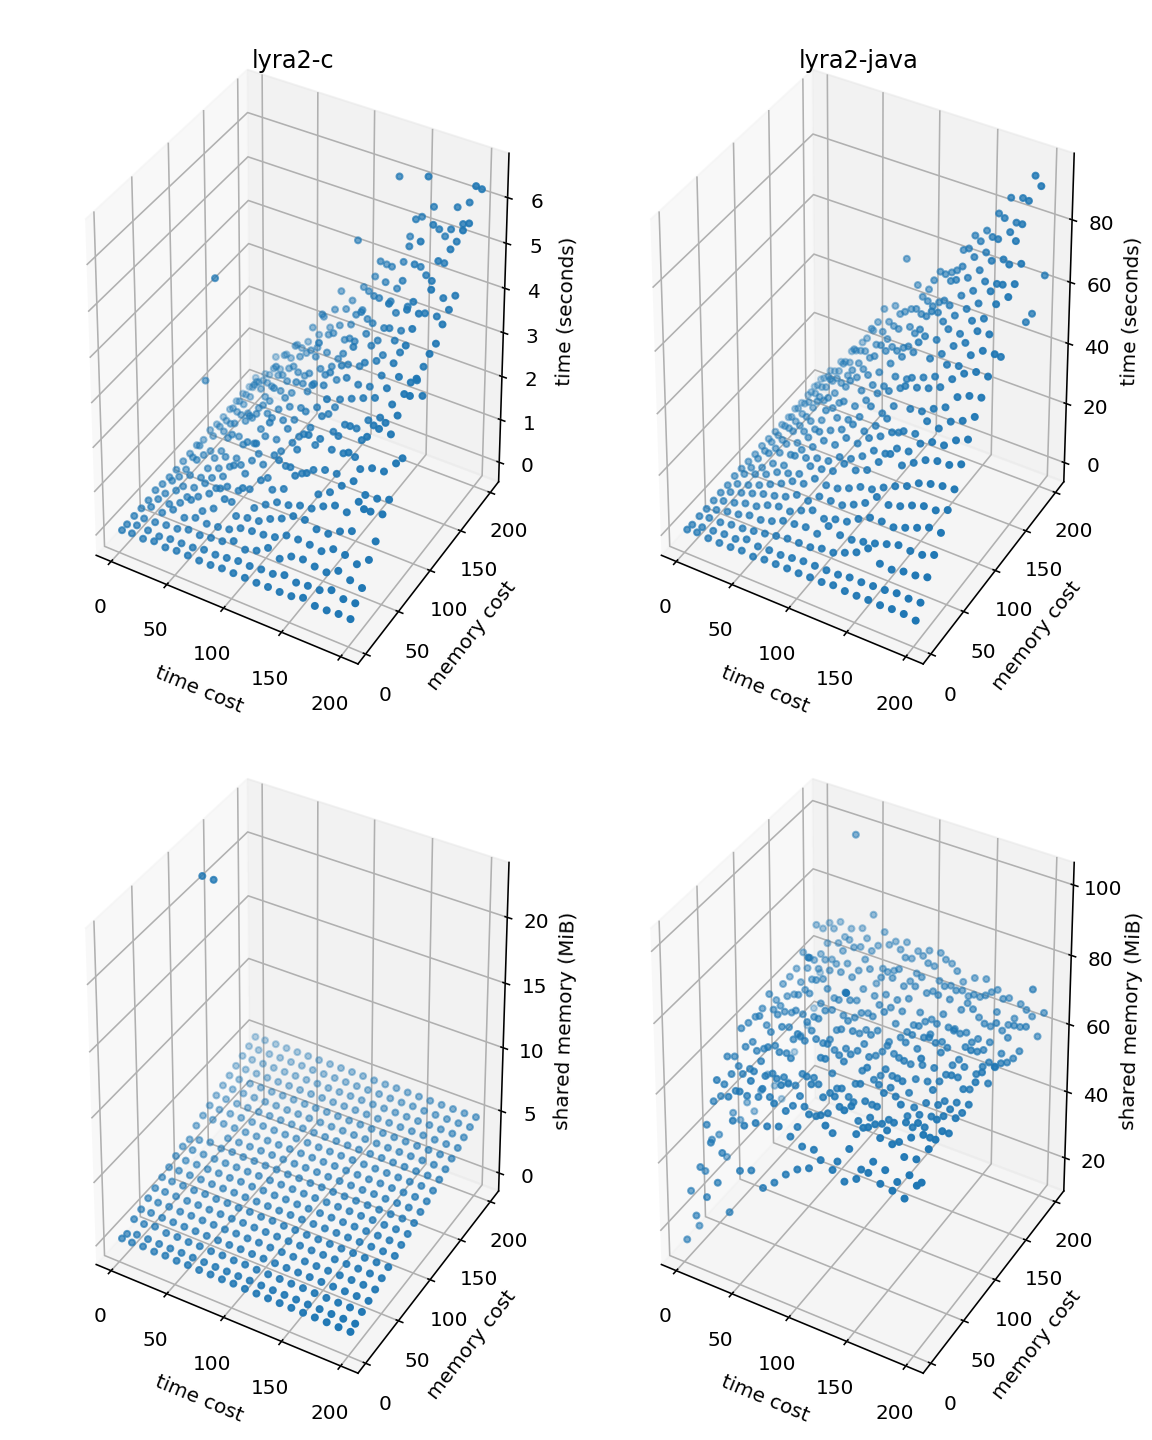
\includegraphics[width=\linewidth,keepaspectratio]{figures/tcost_mcost_blamka_256}
    \caption{\texttt{lyra2-c} compared to \texttt{lyra2-java}: BlaMka sponge, 256 columns. }
    \label{figure:tcost_mcost_blamka_256}
\end{figure}

\begin{figure}[p]
    \centering
    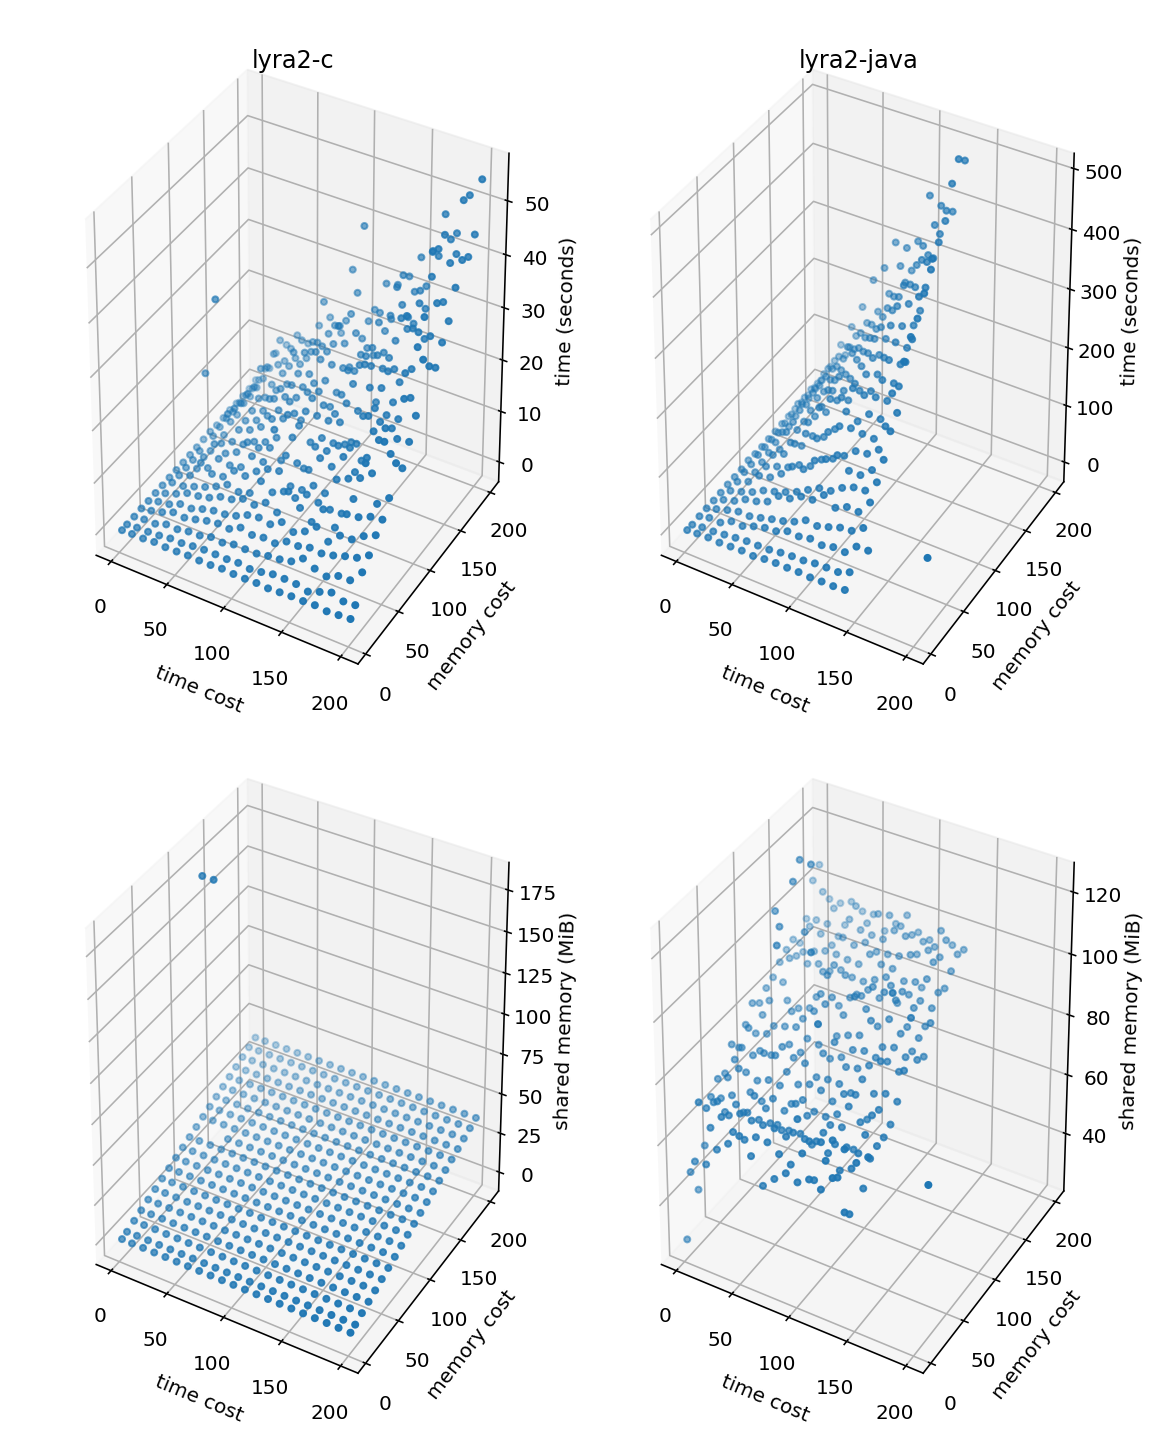
\includegraphics[width=\linewidth,keepaspectratio]{figures/tcost_mcost_blamka_2048}
    \caption{\texttt{lyra2-c} compared to \texttt{lyra2-java}: BlaMka sponge, 2048 columns.}
    \label{figure:tcost_mcost_blamka_2048}
\end{figure}

\clearpage
\subsection{Comparison Conclusion}
\label{sec:comparison-conclusion}

The Java implementation was outperformed by the reference C implementation. This could in part be attributed to language ecosystems or programming skills but it also cannot be denied that the ported version takes a lot of extra steps in order to ensure algorithm-level compatibility. These include the extra rotations requried to simulate little-endian behaviour, as well as simulating pointer arithmetic or unsigned arithmetic for large 64-bit integers.

\section{Android Application}
\label{sec:mobile-application}

Part of the porting effort is a small proof of concept mobile application. This application demonstrates that using a native Java library in an Android project is convenient.

One of the first steps is to determine the minimum versions of Android devices and API levels necessary. Since lyra2-java makes use of unsigned 64-bit number arithmetic, Java 1.8 support is required. This translates into the minimum Android versions of 7.0 and the API level of 24 \footnote{https://developer.android.com/guide/platform/j8-jack.html (visited on 10/23/2017)}.

The most common development environment for Android applications is the Android Studio. Support for Java 1.8 features has not yet landed into the release version of this IDE. So, in order to be able to develop a mobile application with Lyra2, a development version \texttt{3.0} needs to be installed. If you encounter a (similar) traceback as shown in figure \ref{fig:traceback}, there are several possible workarounds available online. The most effective one is to instruct Android Studio to use system libraries:

\begin{minted}{shell}
ANDROID_EMULATOR_USE_SYSTEM_LIBS=1 ./studio.sh
  \end{minted}

\begin{figure}
\begin{minted}{shell}
    Emulator: libGL error: unable to load driver: i965_dri.so
    Emulator: libGL error: driver pointer missing
    Emulator: libGL error: failed to load driver: i965
    Emulator: libGL error: unable to load driver: i965_dri.so
    Emulator: libGL error: driver pointer missing
    Emulator: libGL error: failed to load driver: i965
    Emulator: libGL error: unable to load driver: swrast_dri.so
    Emulator: libGL error: failed to load driver: swrast
    Emulator: X Error of failed request:  BadValue (integer parameter out of range for operation)
    Emulator: Major opcode of failed request:  155 (GLX)
    Emulator: Minor opcode of failed request:  24 (X_GLXCreateNewContext)
    Emulator: Value in failed request:  0x0
    Emulator: Serial number of failed request:  42
    Emulator: Current serial number in output stream:  43
    Emulator: Process finished with exit code 1
\end{minted}
\caption{Android Studio emulator: an obscure error traceback connected to \texttt{libGL}.}
\label{fig:traceback}
\end{figure}

Once these preliminary steps are performed, the development of the application becomes straightforward. Android Studio is based on IntelliJ Studio and therefore picks up lyra2-java from the Maven Central repository in a matter of a couple clicks.

As a result, a simple Android application was developed and is available on GitHub \cite{github:2017:lyra2-mobile}. It consists of a main screen and a results screen. The main screen allows the user to choose the particular configuration of Lyra2. By default, the Blake2b sponge with the time and memory cost of 100 will be used. The password and salt fields are set to the default values of "password" and "salt" respectively, the number of columns is 256 with each column being 12 blocks wide. The permutation inside the sponge makes a total 12 rounds of computations. All of the parameters above can be adjusted.

Figure \ref{fig:lyra2-mobile-demo} demonstrates the hash value after running with default parameters as well as the hash value when using BlaMka instead of Blake2b. The hash values match those from the manual testing section \ref{sec:manual-testing}. In each case the computation lasted for approximately 60 seconds which is consistent with the desktop version times. However, it should be noted that the application was tested in an emulator and not on an actual device.

\begin{figure}[H]
\centering
\begin{subfigure}{.5\textwidth}
  \centering
  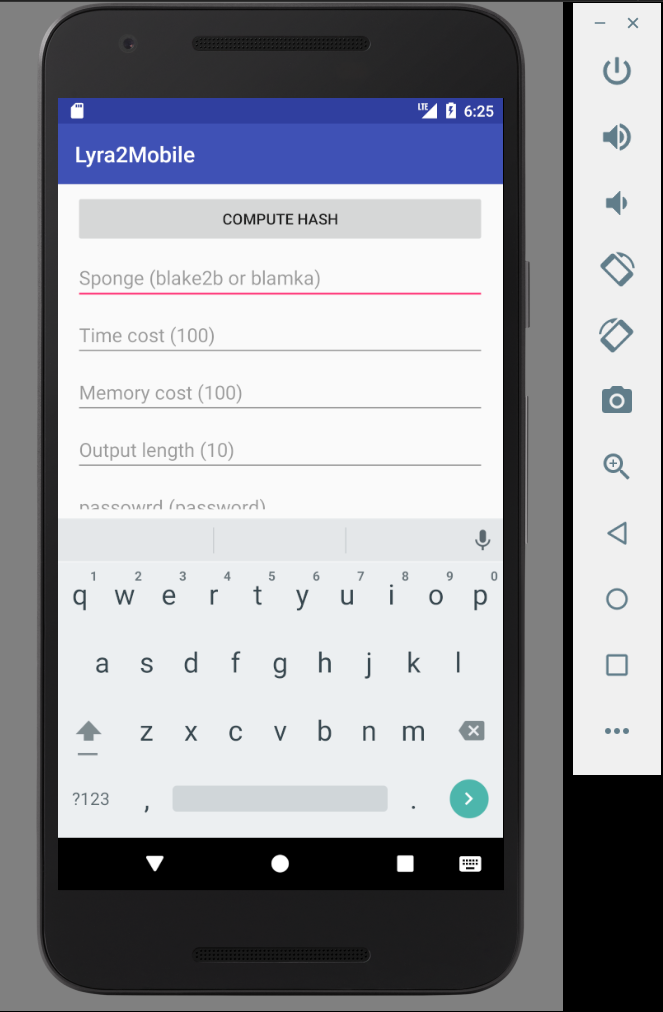
\includegraphics[width=.8\linewidth]{figures/lyra2-mobile-main-clean}
  \caption{Main screen (Blake2b sponge, default)}
  \label{fig:lyra2-mobile-main}
\end{subfigure}%
\begin{subfigure}{.5\textwidth}
  \centering
  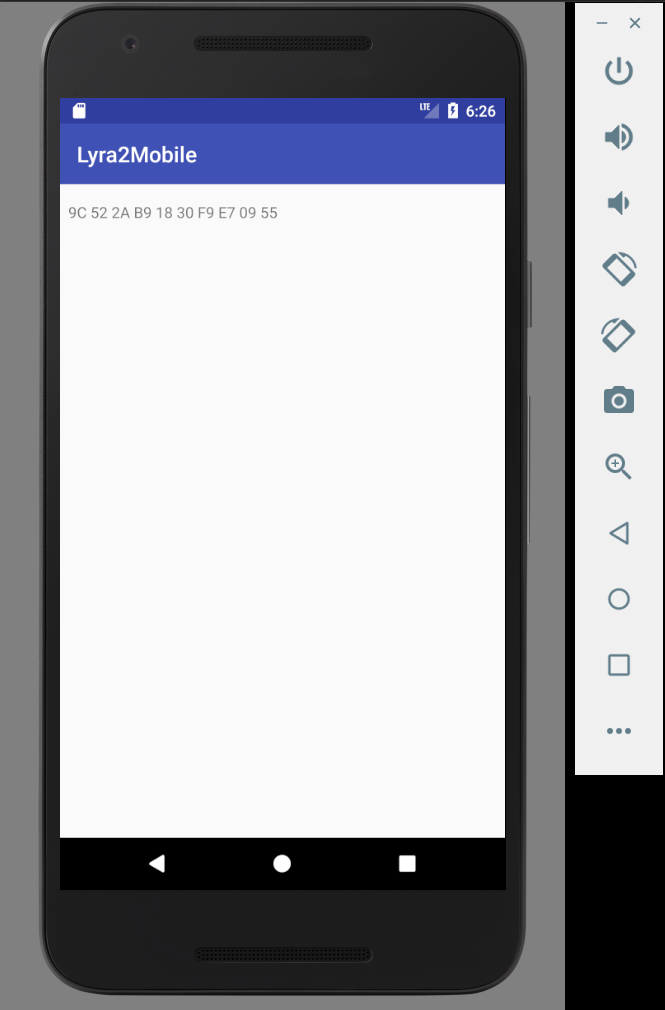
\includegraphics[width=.8\linewidth]{figures/lyra2-mobile-result-clean}
  \caption{Resulting hash (Blake2b sponge, default)}
  \label{fig:lyra2-mobile-result}
\end{subfigure}
\begin{subfigure}{.5\textwidth}
  \centering
  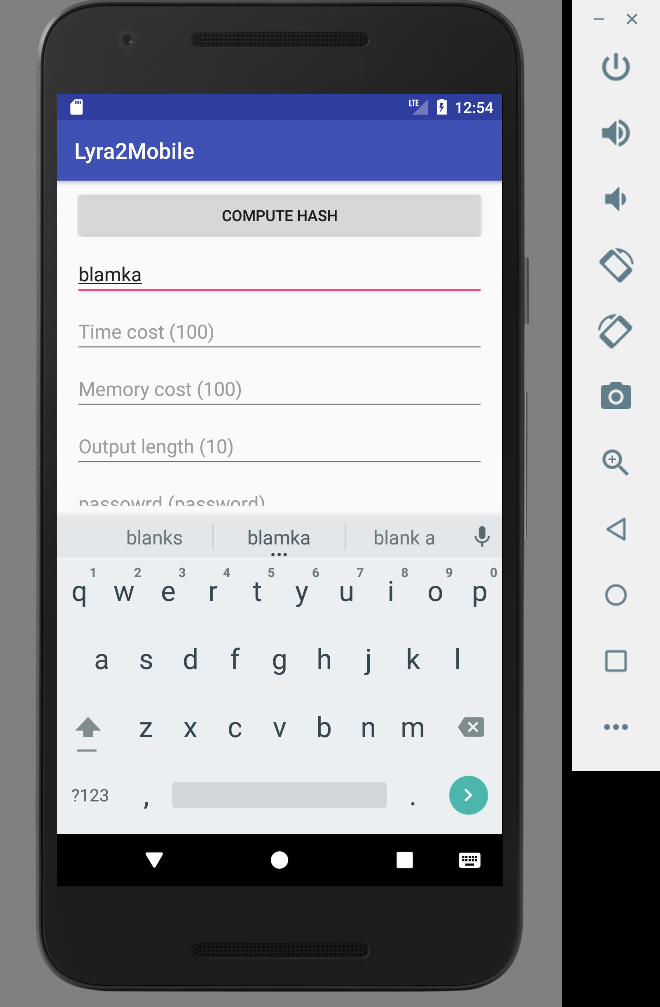
\includegraphics[width=.8\linewidth]{figures/lyra2-mobile-main-blamka-clean}
  \caption{Main screen (BlaMka sponge)}
  \label{fig:lyra2-mobile-main}
\end{subfigure}%
\begin{subfigure}{.5\textwidth}
  \centering
  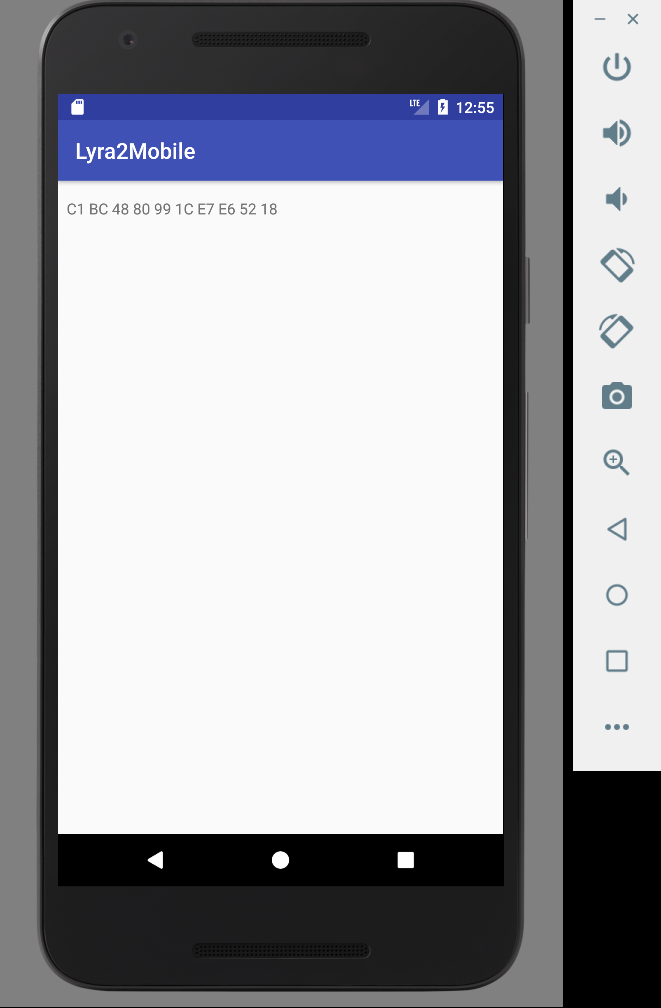
\includegraphics[width=.8\linewidth]{figures/lyra2-mobile-result-blamka-clean}
  \caption{Resulting hash (BlaMka sponge)}
  \label{fig:lyra2-mobile-result}
\end{subfigure}
\caption{Android application running Lyra2. Each of the two configurations runs for \(\approx 60\) seconds. Parameter values on the left, resulting hash in hexadecimal on the right.}
\label{fig:lyra2-mobile-demo}
\end{figure}

\makeatletter\ifthesis@masterthesis
%%%%%%%%%%%%%%%%%%%%%%%%%%%%%%%%%%%%%%%%%%%%%%%%%%%%%%%%%%%%%%%%%%%%%%%%
\chapter{Diskussion}
\label{sec:discussion}
%%%%%%%%%%%%%%%%%%%%%%%%%%%%%%%%%%%%%%%%%%%%%%%%%%%%%%%%%%%%%%%%%%%%%%%%

Den akademischen Wert der Arbeit hervorheben, Vergleich mit verwandten Arbeiten: In welchem Verhältnis stehen die Ergebnisse der Diplomarbeit zu den Ergebnissen anderer Studien? Wo gibt es Unterschiede, wo Gemeinsamkeiten? Warum?

Diskussion offener Punkte, Darstellen der Stärken und Schwächen der vorliegenden Ergebnisse.
\fi\makeatother
%%%%%%%%%%%%%%%%%%%%%%%%%%%%%%%%%%%%%%%%%%%%%%%%%%%%%%%%%%%%%%%%%%%%%%%%
\chapter{Zusammenfassung und Ausblick}
\label{sec:conclusion}
%%%%%%%%%%%%%%%%%%%%%%%%%%%%%%%%%%%%%%%%%%%%%%%%%%%%%%%%%%%%%%%%%%%%%%%%

\makeatletter\ifthesis@masterthesis
Die Zusammenfassung ist nach der Kurzfassung der am häufigsten gelesene Teil, da viele Leser aus Zeitknappheit Arbeiten im Schnellverfahren konsumieren und rasch zur Zusammenfassung blättern. Hier hat man die Chance, dem Leser noch einmal die zentralen Ideen und Ergebnisse der Diplomarbeit zu vermitteln.

Im Gegensatz zur Kurzfassung sind die Leser mit der Problemstellung und der Terminologie bereits vertraut. In der Länge hat man deutlich mehr Spielraum als bei der Kurzfassung, die Zusammenfassung sollte inklusive Ausblick 2 bis max. 10 Seiten umfassen. Hier sollten kompakt die Antworten auf die in der Zielsetzung aufgeworfenen Fragen (Hypothesen) gegeben werden.

Neben einer Zusammenfassung der wichtigsten Ergebnisse sollte auch ein Ausblick gegeben werden: Aufzeigen des Bedarfs an zukünftiger Forschung, potentielle Anwendungsmöglichkeiten der vorgestellten Lösung etc.

In Summe sollte die Zusammenfassung dem Leser die wissenschaftliche und, wenn vorhanden, praktische Relevanz der Arbeit klar und verständlich darlegen.
\fi\makeatother

% insert bibliography and such stuff
\BackMatter

\appendix
\chapter{Android Studio Preview}
\label{chapter:problem?}

At the moment using Lyra2 in an Android application requires a beta (i.e. preview) version of Android Studio. The instructions on the official webpage \footnote{https://developer.android.com/studio/preview/index.html} warn the developer about the need to update plugins. However, this is not the only problem which you may face when running the preview version.

If you require an emulator to test the application, you may be treated with the following  error traceback presented in \ref{fig:traceback}. Different kinds of advice is supposed to help with the problem: preloading the \texttt{libstdc++.so.6} library ahead of time, adding the user who runs Android Studio to the \texttt{video} group, etc. On my machine (a ThinkPad E570 notebook with a dedicated GTX 950M graphics card running ArchLinux), the solution that worked was to instruct Android Studio to rely on system libraries. This can be achieved by setting an environment variable:

\begin{minted}{shell}
ANDROID_EMULATOR_USE_SYSTEM_LIBS=1 ./studio.sh
  \end{minted}

\begin{figure}
\begin{minted}[fontsize=\tiny]{shell}
    Emulator: libGL error: unable to load driver: i965_dri.so
    Emulator: libGL error: driver pointer missing
    Emulator: libGL error: failed to load driver: i965
    Emulator: libGL error: unable to load driver: i965_dri.so
    Emulator: libGL error: driver pointer missing
    Emulator: libGL error: failed to load driver: i965
    Emulator: libGL error: unable to load driver: swrast_dri.so
    Emulator: libGL error: failed to load driver: swrast
    Emulator: X Error of failed request:  BadValue (integer parameter out of range for operation)
    Emulator: Major opcode of failed request:  155 (GLX)
    Emulator: Minor opcode of failed request:  24 (X_GLXCreateNewContext)
    Emulator: Value in failed request:  0x0
    Emulator: Serial number of failed request:  42
    Emulator: Current serial number in output stream:  43
    Emulator: Process finished with exit code 1
\end{minted}
\caption{An obscure error traceback connected to \texttt{libGL}.}
\label{fig:traceback}
\end{figure}


\end{document}
